\documentclass[UTF8]{ctexart}
\usepackage{amsmath}
\usepackage{diagbox}
\usepackage{textcomp}
\usepackage{graphicx}
\usepackage{float}
\usepackage{caption}
\usepackage{adjustbox}
\usepackage{subfigure}
\usepackage{geometry}
\usepackage{pifont}
\begin{document}
\renewcommand{\thefootnote}{\fnsymbol{footnote}}
\newgeometry{left=2cm,bottom=3.5cm,right=2cm}
%\pagestyle{plain}
\linespread{1.4}
\title{\vspace{-5em}\heiti阻尼振动与受迫振动实验报告\vspace{-2.5em}}
\date{}
\maketitle
\begin{center}
{\fangsong 徐浩博\quad 基科01\quad2020010108}
\end{center}

\subsubsection*{摘要}
{\kaishu\normalsize 本实验旨在通过波尔共振仪产生阻尼振动与受迫振动的不同条件,并通过对摆轮在阻尼振动和受迫振动不同条件下的振幅、周期、相位等数据分别进行测量,推导阻尼系数、共振频率、品质因数等,并绘制了幅频、相频特性曲线等图像,使我对有关阻尼振动和受迫振动的相关知识有了更深一步的理解。同时,通过各种曲线的绘制,我还掌握了图线绘制和测量的基本操作和方法,掌握了相关软件的使用方法,并再一次巩固了误差分析和不确定度等相关知识. }
\subsubsection*{关键词:阻尼振动\quad 受迫振动\quad 共振\quad 阻尼系数\quad 品质因数\quad 幅频相频特性曲线\quad暂态过程\vspace{1.5em}}


\section{实验仪器}
波尔共振仪及其控制箱


\section{实验原理及实验数据}
\subsection*{ A) 观测有粘滞阻尼时的阻尼振动规律}
阻尼振动是与速度成正比的电磁作用,若以角度$\theta$作为广义坐标并设正比系数为$\gamma$,则阻尼作用力矩大小可表示为$\theta\frac{\mathrm{d}\theta}{\mathrm{d}t}$,方向与运动方向相反.同时,摆轮还将受到一个系数为$k$的回复力矩. 设摆轮的转动惯量为$I$,则有如下运动方程:
\begin{equation}
I\frac{\mathrm{d}^2\theta}{\mathrm{d}t^2}+k\theta+\gamma\frac{\mathrm{d}\theta}{\mathrm{d}t}=0
\end{equation}
设$\beta=\gamma/2I$,$\omega_0=\sqrt{k/I}$,则运动方程可化为:
\begin{equation}
\ddot{\theta}+2\beta\dot{\theta}+\omega_0^2\theta=0
\end{equation}
其解需要分三种情况讨论:
\paragraph{欠阻尼,$\beta<\omega_0^2$}$\theta=\theta_0e^{-\beta t}cos(\omega_d t+\phi_0)$,其中$\omega_d=\sqrt{\omega_0^2-\beta^2}$;
\paragraph{临界阻尼,$\beta=\omega_0^2$}$\theta=\theta_0e^{-\omega_0t}$;
\paragraph{过阻尼,$\beta>\omega_0^2$}$\theta=e^{-\beta t}(\theta_1e^{\sqrt{\beta^2-\omega_0^2t}}+\theta_2e^{-\sqrt{\beta^2-\omega_0^2t}})$.\par
在这里,由于临界阻尼和过阻尼均不会往复振荡,无震荡周期,故无法利用波尔共振仪进行观测,故我们利用欠阻尼的条件进行实验.
%%%%%%%%%%%%%%
\subsubsection*{A.0 $\beta$的量纲}
下面我们用两种方法推导角度的量纲:\par
1.考虑$\beta=\gamma/2I$,而$M=-\gamma \frac{\mathrm{d}\theta}{\mathrm{d}t}$,力矩$M$量纲为$[M][L]^2[T]^{-2}$,$\frac{\mathrm{d}\theta}{\mathrm{d}t}$量纲为$[T]^{-1}$,故$\gamma$量纲为$[M][L]^2[T]^{-1}$. 而$I$为转动惯量,熟知其量纲为$[M][L]^2$. 综合以上,$\beta$的量纲为$[T]^{-1}$.\par
2.观察方程的解,其中有一项$e^{-\beta t}$,故知$\beta t$为一个无量纲数,则$\beta$的量纲必然为$[T]^{-1}$.
%%%%%%%%%%%%%%%
\subsubsection*{A.1 测量最小阻尼时的阻尼系数$\beta$}
由前述推导,欠阻尼条件下摆轮的运动方程为:
\begin{equation}
\theta=\theta_0e^{-\beta t}cos(\omega_d t+\phi_0)
\label{qianzuni}
\end{equation}
设摆轮振荡周期为$T_d$,初始未满一个周期的时间长度为$t_0$,则其振幅为$\theta_n=\theta_0e^{-\beta(nT_d+t_0)}$. 若要通过测量$T_d$和不同$n$下$\theta_n$的值获得$\beta$的值,则只需对上式取自然对数并线性拟合,得到以下式子:
\begin{equation}
ln\theta_n=ln\theta_0-\beta t_0-n\beta T_d
\end{equation}
则直线斜率为$k=-\beta T_d$
\begin{equation}
\beta=-\frac{k}{T_d}
\end{equation}
考虑到$T_d$较小,测量误差大,故可一次测量十个周期. \par
测量时,首先使波尔共振仪处于工作状态,模式拨至“摆轮”,周期拨至“10”,阻尼置于“0”档,将光电门手动微调避免与摆轮接触. 检查光电门是否位于摆轮长缺口处. 检查完备后,将摆轮拨动使其旋转150°-180°,记录每个周期摆轮的振幅,注意剔除去第一个数据以保证实验数据更精准,记录50次后等待摆轮静止,再拨动摆轮进行5次10周期的测量. 这里需要注意的是,测量周期时拨动幅度应比测量振幅大一些,在接近第一次测量时的振幅后再进行周期测量,以保证周期近似为第一次测量振幅时的周期.\par
对无阻尼档的摆轮阻尼振动时n=1-50时的振幅$\theta_n$进行测量,所得数据如表1所示. 
\begin{table}[H]
{
\centering
\caption{无阻尼挡下阻尼振动n与$\theta_n$数据记录表}\hspace{0mm}
\resizebox{\textwidth}{50mm}{
\begin{tabular}{|c|c|c|c|c|c|c|c|c|c|c|}
\hline
n&1&2&3&4&5&6&7&8&9&10\\
\hline
振幅/°&161&159&158&157&155&155&153&152&151&149\\ 
\hline
ln$\theta$/ln(rad)&1.033&1.021&1.014&1.008&0.995&0.995&0.982&0.976&0.969&0.956\\
\hline
n&11&12&13&14&15&16&17&18&19&20\\
\hline
振幅/°&148&147&146&145&143&142&141&140&139&138\\
\hline
ln$\theta$/ln(rad)&0.949&0.942&0.935&0.929&0.915&0.908&0.901&0.893&0.886&0.879\\
\hline
n&21&22&23&24&25&26&27&28&29&30\\
\hline
振幅/°&137&135&134&133&132&131&130&129&128&127\\
\hline
ln$\theta$/ln(rad)&0.872&0.857&0.850&0.842&0.835&0.827&0.819&0.812&0.804&0.796\\
\hline
n&31&32&33&34&35&36&37&38&39&40\\
\hline
振幅/°&125&125&123&122&121&120&119&118&117&116\\
\hline
ln$\theta$/ln(rad)&0.780&0.780&0.764&0.756&0.748&0.739&0.731&0.722&0.714&0.705\\
\hline
n&41&42&43&44&45&46&47&48&49&50\\
\hline
振幅/°&115&114&113&112&111&110&109&109&107&107\\
\hline
ln$\theta$/ln(rad)&0.697&0.688&0.679&0.670&0.661&0.652&0.643&0.643&0.625&0.625\\
\hline
\end{tabular}}
}
\end{table}

对此组数据利用Excel程序的linest函数对$f$和$n$做最小二乘法直线拟合,设直线斜率为$k$,利用Excel程序的tinv函数计算$p = 0.95$时的$t$因子,可得到:\par
\begin{center}\begin{tabular}{r l}
{斜率}& {$k=-0.008420184$}\\
{斜率标准偏差}& {$s_k=2.99468\times 10^{-5}$}\\
{t因子}& {$t_{0.95,48}=2.010634758$}\\
{斜率不确定度}& {$U_k=t_{0.95,48}\times s_k = 6.021207697\times 10^{-5}$}\\
{斜率相对不确定度}& {$E_k=\frac{U_k}{|k|}=0.7\%$}
\end{tabular}\end{center}
\begin{figure}\centering
{
\caption{无阻尼档下ln$\theta$与$n$拟合曲线}
\label{0}
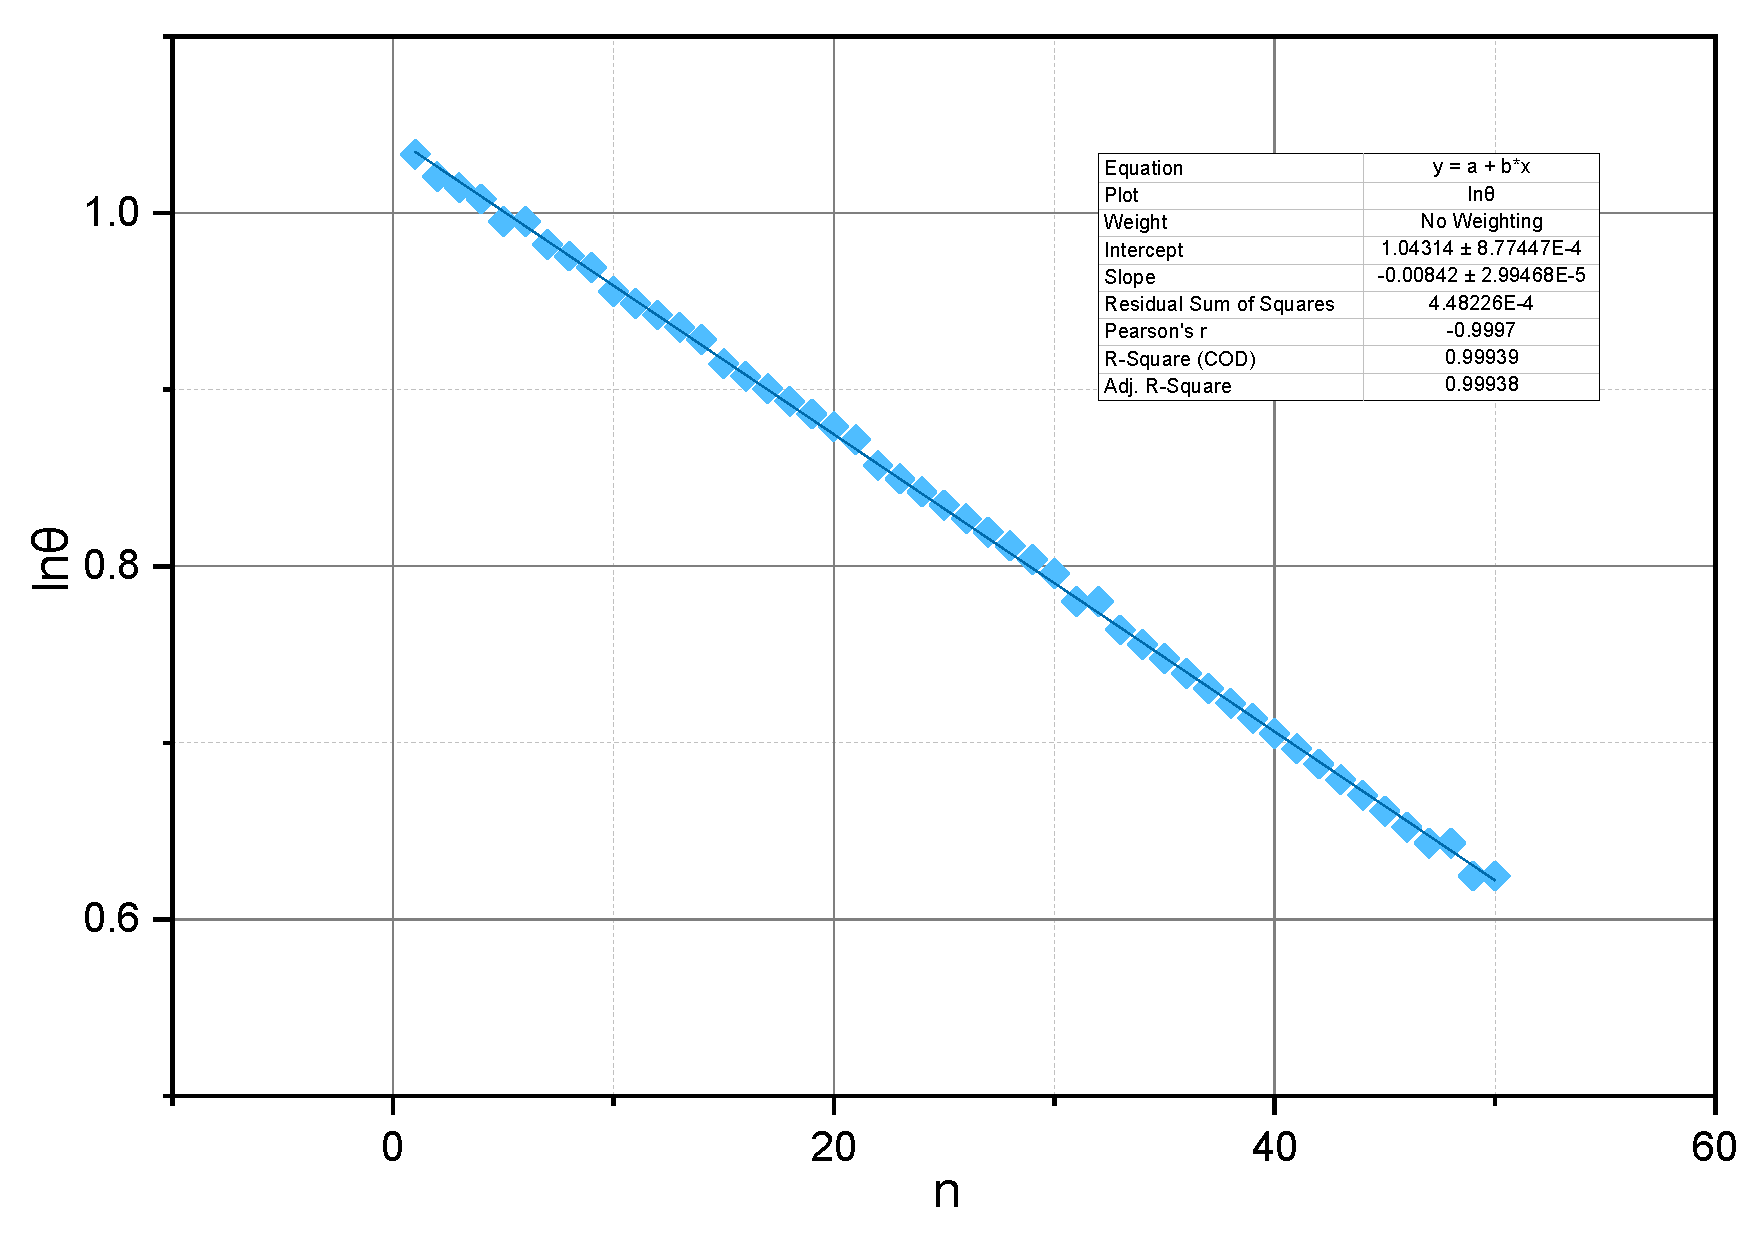
\includegraphics[scale=0.4]{0.pdf}
}
\end{figure}
\begin{table}[H]
{\begin{center}{
\caption{无阻尼档下阻尼振动$T_d$数据记录表}
\begin{tabular}{|c|c|c|c|c|c|}
\hline
测量序号&1&2&3&4&5\\
\hline
$10T_d/s$&14.527&14.550&14.570&14.588&14.605\\
\hline
$T_d/s$&1.4527&1.4550&1.4570&1.4588&1.4605\\
\hline
\end{tabular}}\end{center}}\end{table}
再对每十个振荡周期$10T_d$进行测量并计算出$T_d$,所得数据如表2所示. 对$T_{d}$进行误差分析,可得到:\par
\begin{center}\begin{tabular}{r l}
{$T_{d}$平均值}& {$T_{d}=1.4568s$}\\
{$T_{d}$标准偏差}& {$s_T=0.003073272s$}\\
{t因子}& {$t_{0.95,4}=2.776445105$}\\
{$T_{d}$A类不确定度}& {$U_{TA}=t_{0.95,4}\frac{S_T}{\sqrt{n}}=0.003815971199s$}\\
{$T_{d}$B类不确定度}& {$U_{TB}\approx \Delta_{INS}=0.0002s$}\\
{$T_{d}$不确定度}&{$U_T=\sqrt{U_{TA}^2+U_{TB}^2}=0.00381602361s$}\\
{$T_{d}$相对不确定度}&{$E_T=\frac{U_T}{T_{d}}=0.3\%$}
\end{tabular}\end{center}
最后由(5)式$\beta=-\frac{k}{T_{d}}$计算$\beta$及其不确定度
\begin{center}\begin{tabular}{r l}
{阻尼系数}& {$\beta=0.0057799s^{-1}$}\\
{阻尼系数相对不确定度}&{$E_{\beta}=\sqrt{E_k^2+E_T^2}=0.8\%$}\\
{阻尼系数不确定度}&{$s_{\beta}=\beta\times E_{\beta}=0.0000462s^{-1}$}
\end{tabular}\end{center}
则实验最终测得的阻尼系数为$(5.780\pm0.046)\times10^{-3}s^{-1}$.\footnote{由于书中所写“约定不确定度为0.0002s”意义模糊,此处我将其理解为$T_d$的B类不确定度为0.0002s. 这一点是有道理的,因为经过计算,我们发现$T_d$的A类不确定度远大于0.0002s,相比而言B类不确定度更像一个小量.下同.\par 若我们认为$T_d$的总不确定度为0.0002s,则$E_T=0.01\%$,$E_{\beta}=\sqrt{E_k^2+E_T^2}=0.7\%$,$s_{\beta}=0.040s^{-1}$,最终阻尼系数为$(5.780\pm0.040)\times10^{-3}s^{-1}$.}
%%%%%%%%%%%%%%
\subsubsection*{A.2 利用阻尼系数$\beta$和振动周期$T_d$计算固有角频率$\omega_0$}
由上一小问,我们得到$T_{10}=14.568s$,从而振动周期$T_d=\frac{T_{10}}{10}=1.4568s$,故振动角频率$\omega_d=\frac{2\pi}{T_d}=4.3130s^{-1}$.\par
由原理部分的推导,我们有
\begin{equation}
\omega_d=\sqrt{\omega_0^2-\beta^2}
\end{equation}
由此得到$\omega_0=\sqrt{\omega_d^2+\beta^2}=4.3130s^{-1}$. 这表明,在阻尼很小的情况下,振动角频率$\omega_d$与固有角频率$\omega_0$数值大致相等,可以用前者代替后者.

\subsubsection*{A.3 测量其他两种阻尼状态的振幅}
我们依然采用A.2中的测量步骤及方法对阻尼2、3档的阻尼系数阻尼系数$\beta$进行测量.
考虑到有阻尼时振动会很快停止,因此我们测量一个周期的时间. \par
测量时基本步骤同A.1,首先使波尔共振仪处于工作状态,模式拨至“摆轮”,周期拨至“1”,阻尼置于对应档,再仿照A.1的基本步骤进行测量.\par
\paragraph{对阻尼2档的数据测量及分析如下:}\quad \par

对阻尼2档下的摆轮阻尼振动n=1-10时的振幅$\theta_n$进行测量,所得数据如表5所示. 
\begin{table}[H]
{
\centering
\caption{阻尼2档下阻尼振动$n$与$\theta_n$数据记录表}\hspace{15mm}
%\resizebox{\textwidth}{40mm}{
\begin{tabular}{|c|c|c|c|c|c|c|c|c|c|c|}
\hline
n&1&2&3&4&5&6&7&8&9&10\\
\hline
振幅/°&171&154&141&129&118&108&99&91&83&76\\ 
\hline
ln$\theta$/ln(rad)&1.093&0.989&0.901&0.812&0.723&0.634&0.547&0.463&0.371&0.283\\
\hline
\end{tabular}}%}
\end{table}

对此组数据利用Excel程序的linest函数对$f$和$n$做最小二乘法直线拟合,设直线斜率为$k$,利用Excel程序的tinv函数计算$p = 0.95$时的$t$因子,可得到:\par
\begin{center}\begin{tabular}{r l}
{斜率}& {$k=-0.08907448$}\\
{斜率标准偏差}& {$s_k=5.65677\times 10^{-4}$}\\
{t因子}& {$t_{0.95,8}=2.306004135$}\\
{斜率不确定度}& {$U_k=t_{0.95,8}\times s_k = 1.304454\times 10^{-3}$}\\
{斜率相对不确定度}& {$E_k=\frac{U_k}{|k|}=1\%$}
\end{tabular}\end{center}
\begin{figure}\centering
{
\caption{阻尼2档下ln$\theta$与$n$拟合曲线}
\label{2_linear}
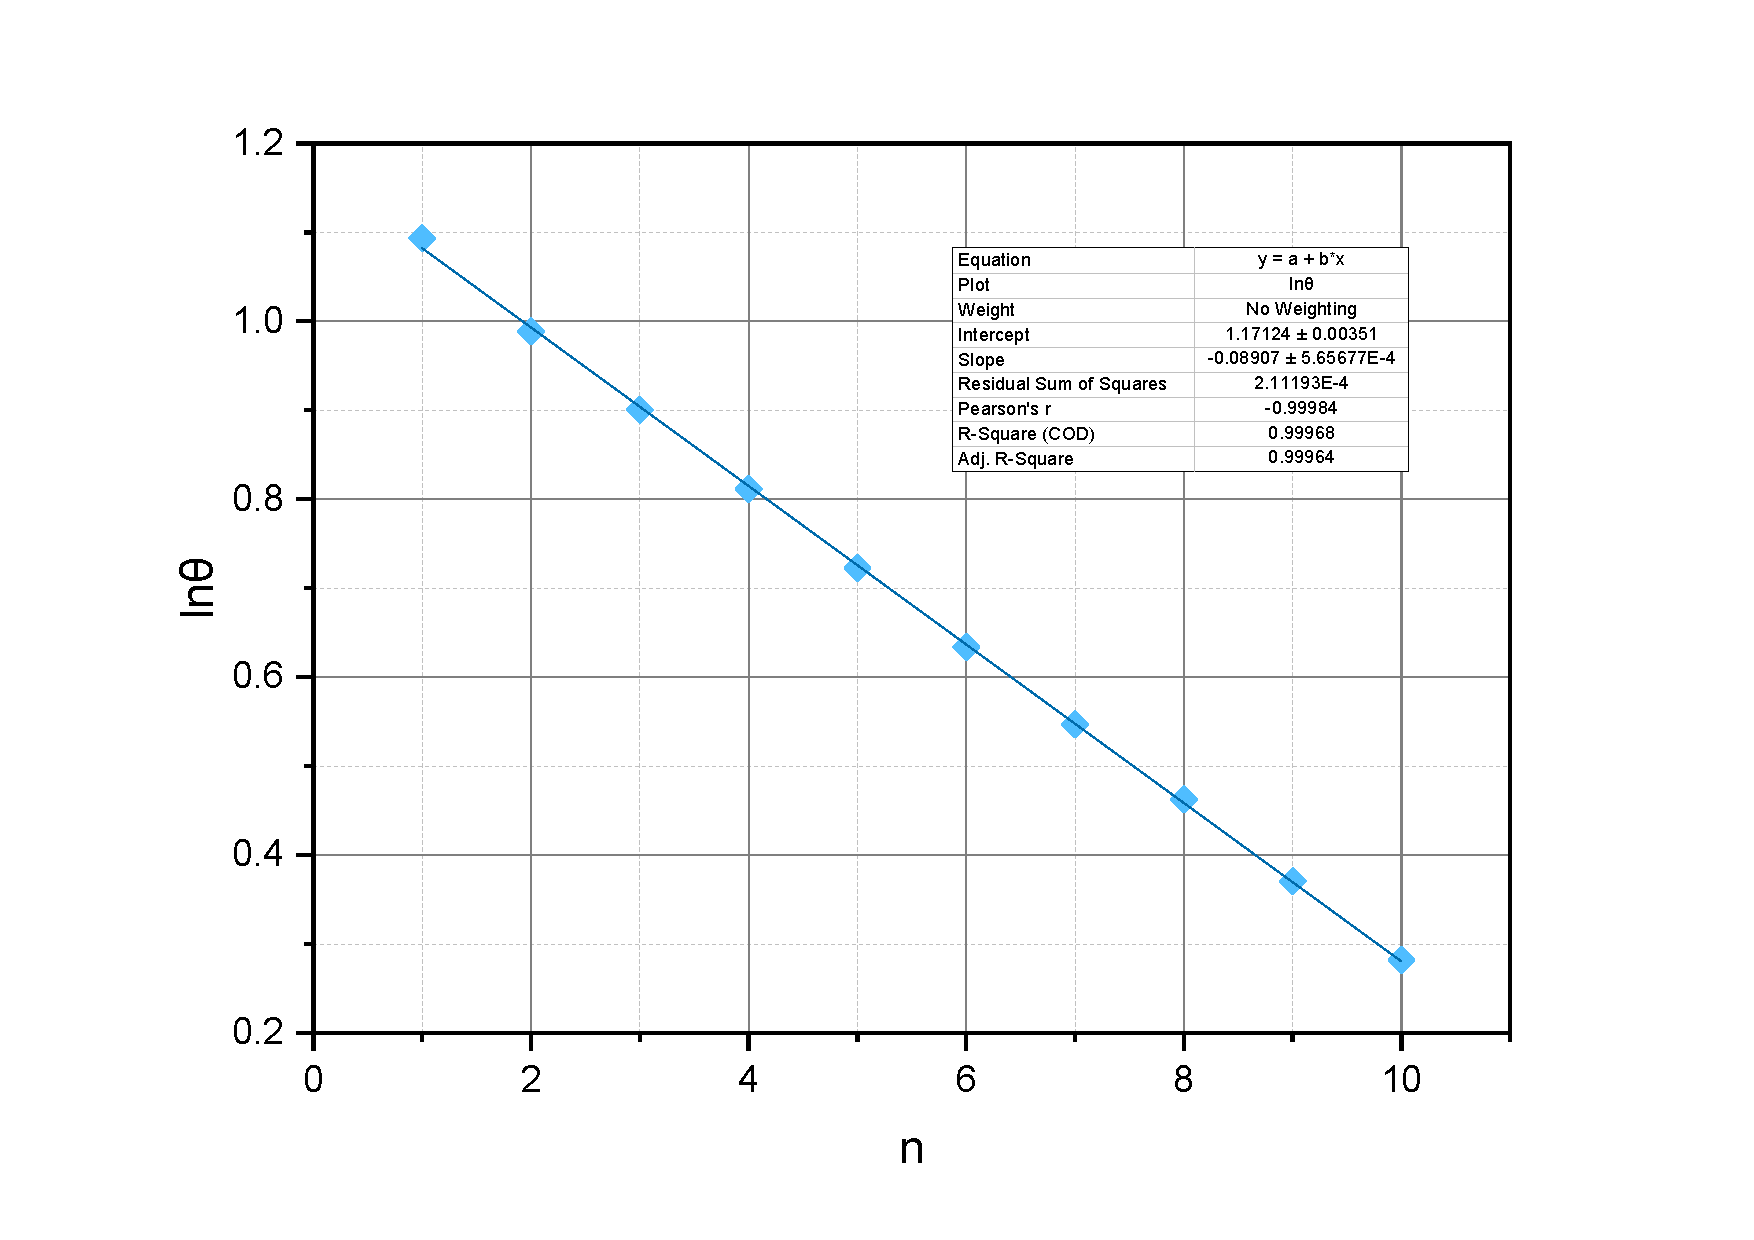
\includegraphics[scale=0.4]{2_linear.pdf}
}
\end{figure}
再对阻尼2档下振荡周期$T_{d}$进行测量,所得数据如表6所示. 
\begin{table}[H]
{\begin{center}{
\caption{阻尼2档下阻尼振动$T_d$数据记录表}
\begin{tabular}{|c|c|c|c|c|c|}
\hline
测量序号&1&2&3&4&5\\
\hline
$T_d/s$&1.456&1.457&1.459&1.460&1.460\\
\hline
\end{tabular}}\end{center}}\end{table}
对$T_{d}$进行误差分析,可得到:\par
\begin{center}\begin{tabular}{r l}
{$T_{d}$平均值}& {$T_{d}=1.458s$}\\
{$T_{d}$标准偏差}& {$s_T=1.8165902\times 10^{-3}s$}\\
{t因子}& {$t_{0.95,4}=2.776445105$}\\
{$T_{d}$A类不确定度}& {$U_{TA}=t_{0.95,4}\frac{S_T}{\sqrt{n}}=2.2555594651\times 10^{-3}s$}\\
{$T_{d}$B类不确定度}& {$U_{TB}\approx \Delta_{INS}=0.002s$}\\
{$T_{d}$不确定度}&{$U_T=\sqrt{U_{TA}^2+U_{TB}^2}=3.01458243\times 10^{-3}s$}\\
{$T_{d}$相对不确定度}&{$E_T=\frac{U_T}{T_{d}}=0.2\%$}
\end{tabular}\end{center}
最后由(5)式$\beta=-\frac{k}{T_{d}}$计算$\beta$及其不确定度
\begin{center}\begin{tabular}{r l}
{阻尼系数}& {$\beta=0.06109360768s^{-1}$}\\
{阻尼系数相对不确定度}&{$E_{\beta}=\sqrt{E_k^2+E_T^2}=1\%$}\\
{阻尼系数不确定度}&{$s_{\beta}=\beta\times E_{\beta}=0.0006s^{-1}$}
\end{tabular}\end{center}
则实验最终测得的2档阻尼系数为$(6.11\pm0.06)\times10^{-2}s^{-1}$.\footnote{ 若我们认为$T_d$的总不确定度为0.002s,则$E_T=0.1\%$,$E_{\beta}=\sqrt{E_k^2+E_T^2}=1\%$,$s_{\beta}=0.0006s^{-1}$,最终阻尼系数为$(6.11\pm0.06)\times10^{-2}s^{-1}$.}
此值远小于$\omega_d=\frac{2\pi}{T_d}=4.309s^{-1}$,故也可以用阻尼振动角频率$\omega_d$代替固有角频率$\omega_0$.


\paragraph{对阻尼3档的数据测量及分析如下:}\quad \par
对阻尼3档下的摆轮阻尼振动n=1-10时的振幅$\theta_n$进行测量,所得数据如表5所示. 
\begin{table}[ht]
{
\centering
\caption{阻尼3档下阻尼振动$n$与$\theta_n$数据记录表}\hspace{15mm}
%\resizebox{\textwidth}{40mm}{
\begin{tabular}{|c|c|c|c|c|c|c|c|c|c|c|}
\hline
n&1&2&3&4&5&6&7&8&9&10\\
\hline
振幅/°&158&139&123&108&95&83&73&64&56&49\\ 
\hline
ln$\theta$/ln(rad)&1.014&0.886&0.764&0.634&0.506&0.371&0.242&0.111&-0.023&-0.156\\
\hline
\end{tabular}}%}
\end{table}

对此组数据利用Excel程序的linest函数对$f$和$n$做最小二乘法直线拟合,设直线斜率为$k$,利用Excel程序的tinv函数计算$p = 0.95$时的$t$因子,可得到:\par
\begin{center}\begin{tabular}{r l}
{斜率}& {$k=-0.13016598$}\\
{斜率标准偏差}& {$s_k=4.94189\times 10^{-4}$}\\
{t因子}& {$t_{0.95,8}=2.306004135$}\\
{斜率不确定度}& {$U_k=t_{0.95,8}\times s_k = 1.139601877\times 10^{-3}$}\\
{斜率相对不确定度}& {$E_k=\frac{U_k}{|k|}=0.8\%$}
\end{tabular}\end{center}
\begin{figure}\centering
{
\caption{阻尼3档下ln$\theta$与$n$拟合曲线}
\label{3_linear}
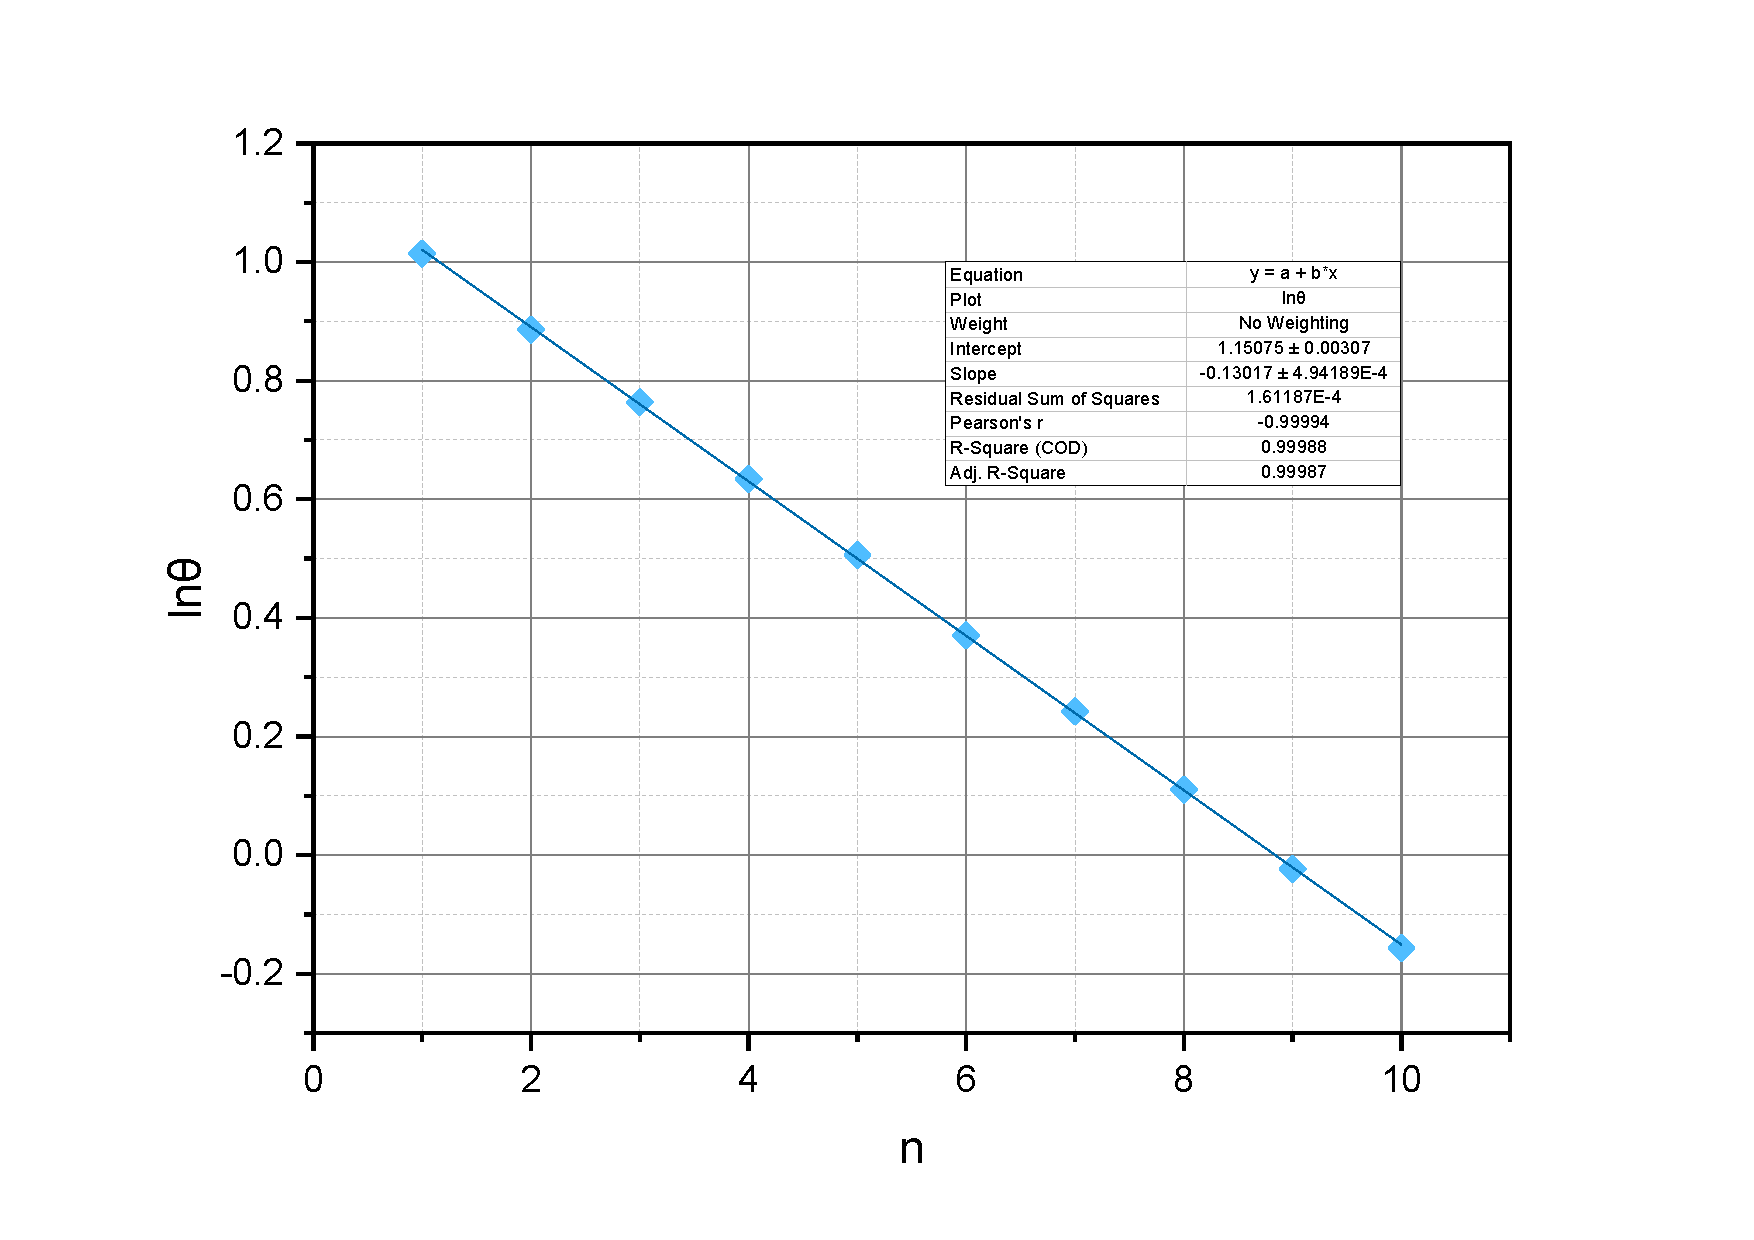
\includegraphics[scale=0.4]{3_linear.pdf}
}
\end{figure}
再对阻尼3档下振荡周期$T_{d}$进行测量,所得数据如表6所示. 
\begin{table}[H]
{\begin{center}{
\caption{阻尼3档下阻尼振动$T_d$数据记录表}
\begin{tabular}{|c|c|c|c|c|c|}
\hline
测量序号&1&2&3&4&5\\
\hline
$T_d/s$&1.453&1.455&1.457&1.457&1.460\\
\hline
\end{tabular}}\end{center}}\end{table}
对$T_{d}$进行误差分析,可得到:\par
\begin{center}\begin{tabular}{r l}
{$T_{d}$平均值}& {$T_{d}=1.456s$}\\
{$T_{d}$标准偏差}& {$s_T=2.6076809\times 10^{-3}s$}\\
{t因子}& {$t_{0.95,4}=2.776445105$}\\
{$T_{d}$A类不确定度}& {$U_{TA}=t_{0.95,4}\frac{S_T}{\sqrt{n}}=3.23786349\times 10^{-3}s$}\\
{$T_{d}$B类不确定度}& {$U_{TB}\approx \Delta_{INS}=0.002s$}\\
{$T_{d}$不确定度}&{$U_T=\sqrt{U_{TA}^2+U_{TB}^2}=3.80575353\times 10^{-3}s$}\\
{$T_{d}$相对不确定度}&{$E_T=\frac{U_T}{T_{d}}=0.2\%$}
\end{tabular}\end{center}
最后由(5)式$\beta=-\frac{k}{T_{d}}$计算$\beta$及其不确定度
\begin{center}\begin{tabular}{r l}
{阻尼系数}& {$\beta=0.08939971154s^{-1}$}\\
{阻尼系数相对不确定度}&{$E_{\beta}=\sqrt{E_k^2+E_T^2}=0.8\%$}\\
{阻尼系数不确定度}&{$s_{\beta}=\beta\times E_{\beta}=0.0007s^{-1}$}
\end{tabular}\end{center}
则实验最终测得的3档阻尼系数为$(8.94\pm0.07)\times10^{-2}s^{-1}$.\footnote{ 若我们认为$T_d$的总不确定度为0.002s,则$E_T=0.1\%$,$E_{\beta}=\sqrt{E_k^2+E_T^2}=0.8\%$,$s_{\beta}=0.0007s^{-1}$,最终阻尼系数为$(8.94\pm0.07)\times10^{-2}s^{-1}$.}
此值远小于$\omega_d=\frac{2\pi}{T_d}=4.315s^{-1}$,故也可以用阻尼振动角频率$\omega_d$代替固有角频率$\omega_0$.
%%%%%%%%%%%%%%%%%%%%%%%%%%

\subsubsection*{A.4 计算三种阻尼状态下的品质因数$Q$}
品质因数$Q$可以衡量振动系统的能耗比例,定义为:
\begin{equation}
Q=\frac{2\pi E}{|\Delta E|}
\end{equation}
可以看出,阻尼越小,耗能百分比越低,品质因数$Q$越高. 对于$\beta \ll \omega_0$的欠阻尼情况,由(\ref{qianzuni})式,有
\begin{equation}\begin{split}
\dot{\theta}=-\theta_0 e^{-\beta t}[\beta \cos(\omega_d t+\phi_0)+\omega_d \sin(\omega_dt+\phi_0)]\\
\approx -\theta_0 e^{-\beta t}\omega_0 \sin(\omega_dt+\phi_0)
\end{split}\end{equation}
从而
\begin{equation}
E=E_p+E_k=\frac{1}{2}k\theta^2+\frac{1}{2}J\dot{\theta}^2=\frac{1}{2}k\theta_0^2e^{-2\beta t}
\end{equation}
则品质因数
\begin{equation}
Q=2\pi\frac{E}{|\Delta E|}=2\pi\frac{E}{E(1-e^{-2\beta T})}\approx \frac{2\pi}{2\beta T_0}=\frac{\omega_0}{2\beta}
\label{Q}
\end{equation}
则已知阻尼系数$\beta$和固有角频率$\omega_0$即可计算出对应条件下的$Q$,而由前述分析,在阻尼系数较小时可以用$\omega_d$代替$\omega_0$,故$\displaystyle{Q=\frac{\omega_0}{2\beta}=\frac{\pi}{\beta T_d}}$
\paragraph{对无阻尼档的分析如下:}\quad \par
无阻尼档时$\beta=5.780\times 10^{-3}s^{-1}$,$T_d=1.4568s$,则$Q_0=\frac{\pi}{\beta T_d}=373.1$.\par

\paragraph{对阻尼2档的分析如下:}\quad \par
阻尼2档时$\beta=6.11\times 10^{-2}s^{-1}$,$T_d=1.458s$,则$Q_2=\frac{\pi}{\beta T_d}=35.3$.\par

\paragraph{对阻尼3档的分析如下:}\quad \par
阻尼3档时$\beta=8.93\times 10^{-2}s^{-1}$,$T_d=1.456s$,则$Q_3=\frac{\pi}{\beta T_d}=24.2$.\par

\subsection*{ B) 分析振动系统受迫振动的基本规律,观测幅频特性}
受迫振动是振动在周期性外力的推动下发生的一种振动过程,与上面讨论的阻尼振动相比,它的受力多了周期性强迫力. 由于波尔共振仪的特殊结构,连杆、摇杆远长度远大于偏心轮偏心半径,则电机匀速转动可以提供给卷形弹簧简谐激励. 在角频率$\omega$、振幅$A_D$的简谐信号激励下,其轨迹为$A_D\cos(\omega t)$,则摆轮位移为$\theta$时,弹簧转角为$\theta-A_D\cos(\omega t)$,再乘以系数$k$即为恢复力矩,则运动方程改写为:
\begin{equation}
I\frac{\mathrm{d}^2\theta}{\mathrm{d}t^2}+k(\theta-A_D\cos(\omega t))+\gamma\frac{\mathrm{d}\theta}{\mathrm{d}t}=0
\end{equation}
在欠阻尼的条件下可以将通解表示为:
\begin{equation}
\theta=\theta_0e^{-\beta t}\cos(\sqrt{\omega_0^2-\beta^2}t+\phi_0)+\theta_m\cos(\omega t-\phi)\label{tongjie}
\end{equation}
其中前一项在时间远大于弛豫时间后趋于零,运动表现为后一项的特征. 后一项为该非齐次微分方程特解,其中常数为:
\begin{equation}
\theta_m=\frac{\omega_0^2A_D}{\sqrt{(\omega_0^2-\omega^2)^2+(2\beta\omega)^2}}
\label{theta}
\end{equation}
\begin{equation}
\phi=\arctan\frac{2\beta\omega}{\omega_0^2-\omega^2}
\label{phi}
\end{equation}
\subsubsection*{B.1 弱阻尼下受迫振动相关物理量的推导}
由(\ref{theta})式知,只需$(\omega_0^2-\omega^2)^2+(2\beta\omega)^2=\omega^4+(4\beta^2-2\omega_0^2)\omega^2+\omega_0^4$取最小值时振幅有最大值,由二次函数的性质,$\omega=\sqrt{\omega_0^2-2\beta^2}$时振幅有最大值. 设共振频率为$\omega_{res}$,共振处振幅为$\theta_{res}$,相位差为$\phi_{res}$,则有
\begin{equation}\omega_{res}=\sqrt{\omega_0^2-2\beta^2}\label{omegares}\end{equation}
\begin{equation}\theta_{res}=\frac{\omega_0^2A_D}{2\beta\sqrt{\omega_0^2-\beta^2}}\end{equation}
\begin{equation}\phi_{res}=\frac{\sqrt{\omega_0^2-2\beta^2}}{\beta}\end{equation}\par
由(\ref{Q})式得:$\displaystyle{Q=\frac{2\pi}{1-e^{-2\beta T_d}}=\frac{2\pi}{1-e^{-\beta\frac{2\pi}{\sqrt{\omega_0^2-\beta^2}}}}}$,可以看出随着$\displaystyle{\frac{\omega_0}{\beta}}$增大,$Q$也增大,而$\displaystyle{\theta_{res}=\frac{\omega_0^2A_D}{2\beta\sqrt{\omega_0^2-\beta^2}}                                                                                                                                                                                                                          }$也增大. 即品质因数$Q$与共振处振幅$\theta_{res}$成正相关的关系. 这种关系在$\beta$较小的弱阻尼条件下会更加明显. 在弱阻尼条件下,有$\displaystyle{Q\approx \frac{\omega_0}{2\beta}}$,则$\displaystyle{\theta_{res}=\frac{2Q^2A_D}{\sqrt{4Q^2-1}}}$,显然有正相关关系.\par
在弱阻尼条件下,$\beta\ll \omega_0$,则由(\ref{omegares})式,有$\omega_{res}\approx\omega_0$,这说明了弱阻尼状态下,共振频率近似等于振动系统的固有频率.
%%%%%%%%%%%%%%%%%%%%%%%%%%%%%%%
\subsubsection*{B.2 判断受迫振动达到了稳态的方法}
\paragraph{1.估算时间常数$\tau$}在(\ref{tongjie})式中,通解项$\theta_0e^{-\beta t}\cos(\sqrt{\omega_0^2-\beta^2}t+\phi_0)$中的指数项$e^{-\beta t}$导致衰减,则其时间常数$\tau=1/\beta$. 由前述计算,我们取$\beta\approx0.1s^{-1}$,则$\tau=10s$,在五倍时间常数下,我们可以近似认为达到稳态,因为共振幅度数量级大约为($1\times10^2$)°,则五倍时间常数(50s)后小于1°(仪器最小分度值),可以认为达到稳态.
\paragraph{2.观察振幅和相位差}初始时振幅变化极快,在变化减缓,如连续几个周期无改变时,通过振幅改变观察是否达到稳态较为困难,这时可以通过闪光灯观察相位差来判断是否达到稳态. 考虑到 (\ref{tongjie})式中,若通解项比起特解项的值仍不可忽略,则会显著产生相位差的改变.
%%%%%%%%%%%%%%%%%%%%%%%%%%%%%%%
\subsubsection*{B.3 测试幅频特性和相频特性}
测量时,首先使波尔共振仪处于工作状态,模式拨至“强迫力”,周期拨至“1”,阻尼置于对应档,将光电门手动微调避免与摆轮或刻度盘接触. 检查摆轮处的光电门是否位于摆轮长缺口处,并调节刻度盘,使白线恰好位于0和180°. 检查完备后,根据A中的计算出的阻尼振动角频率(已证明共振频率约等于阻尼振动角频率)在其周围附近调节强迫激励周期旋钮以改变点击运动角频率. 要注意,共振频率附近测量应密集一些,且频率的选择应关于共振频率大致对称. 每次频率调整后,待受迫振动达到稳态,记录振幅和相位差. 这里相位差可以采用两次取平均的方法获得.\par
\paragraph{对阻尼2档的数据测量及分析如下:}\quad \par
阻尼2档下测量的数据如下表所示,据此可以画出阻尼2档下的幅频特性曲线和相频特性曲线. 这里利用OriginPro程序,在作出散点图后,用B-spline算法对散点间的连线进行平滑化处理,得到平滑曲线.\par
\begin{table}[H]{\begin{center}\caption{阻尼2档不同强迫力频率下受迫振动数据记录表}%\label{temp1}\resizebox{\textwidth}{!}{
\begin{tabular}[H]{|c|c|c|c|c|c|c|c|c|}
\hline
次数&1&2&3&4&5&6&7&8\\
\hline
强迫力周期$T_F/s$&1.370&1.390&1.410&1.430&1.440&1.445&1.450&1.455\\
\hline
强迫力频率$\omega_F/s^{-1}$&4.586&4.520&4.456&4.394&4.363&4.348&4.333&4.318\\
\hline
摆轮振幅$\theta$/°&31&39&50&77&108&130&142&146\\
\hline
相位差1$\phi_1$/°&164.5&162.0&158.0&147.0&132.0&117.0&102.0&88.0\\
\hline
相位差2$\phi_2$/°&167.0&163.0&160.5&148.5&133.5&118.0&102.5&88.5\\
\hline
平均相位差$\phi$/°&165.8&162.5&159.3&147.8&132.8&117.5&102.3&88.3\\
\hline
平均相位差$\phi$/rad&2.893&2.836&2.779&2.579&2.317&2.051&1.785&1.540\\
\hline
次数&9&10&11&12&13&14&15&16\\
\hline
强迫力周期$T_F/s$&1.460&1.465&1.470&1.480&1.490&1.510&1.530&1.550\\
\hline
强迫力频率$\omega_F/s^{-1}$&4.304&4.289&4.274&4.245&4.217&4.161&4.107&4.054\\
\hline
摆轮振幅$\theta$/°&144&133&123&109&93&67&50&35\\
\hline
相位差1$\phi_1$/°&74.0&66.0&56.0&45.0&35.0&23.5&16.0&12.0\\
\hline
相位差2$\phi_2$/°&74.5&66.5&57.0&46.0&36.5&25.5&18.5&15.5\\
\hline
平均相位差$\phi$/°&74.3&66.3&56.5&45.5&35.8&24.5&17.3&13.8\\
\hline
平均相位差$\phi$/rad&1.296&1.156&0.986&0.794&0.624&0.428&0.301&0.240\\
\hline
\end{tabular}%}
\end{center}}\end{table}

\begin{figure}[H]\centering
{
\newgeometry{a4paper,left=0cm,right=1cm}\hspace{-20mm}
\subfigure[阻尼2档下幅频特性曲线]{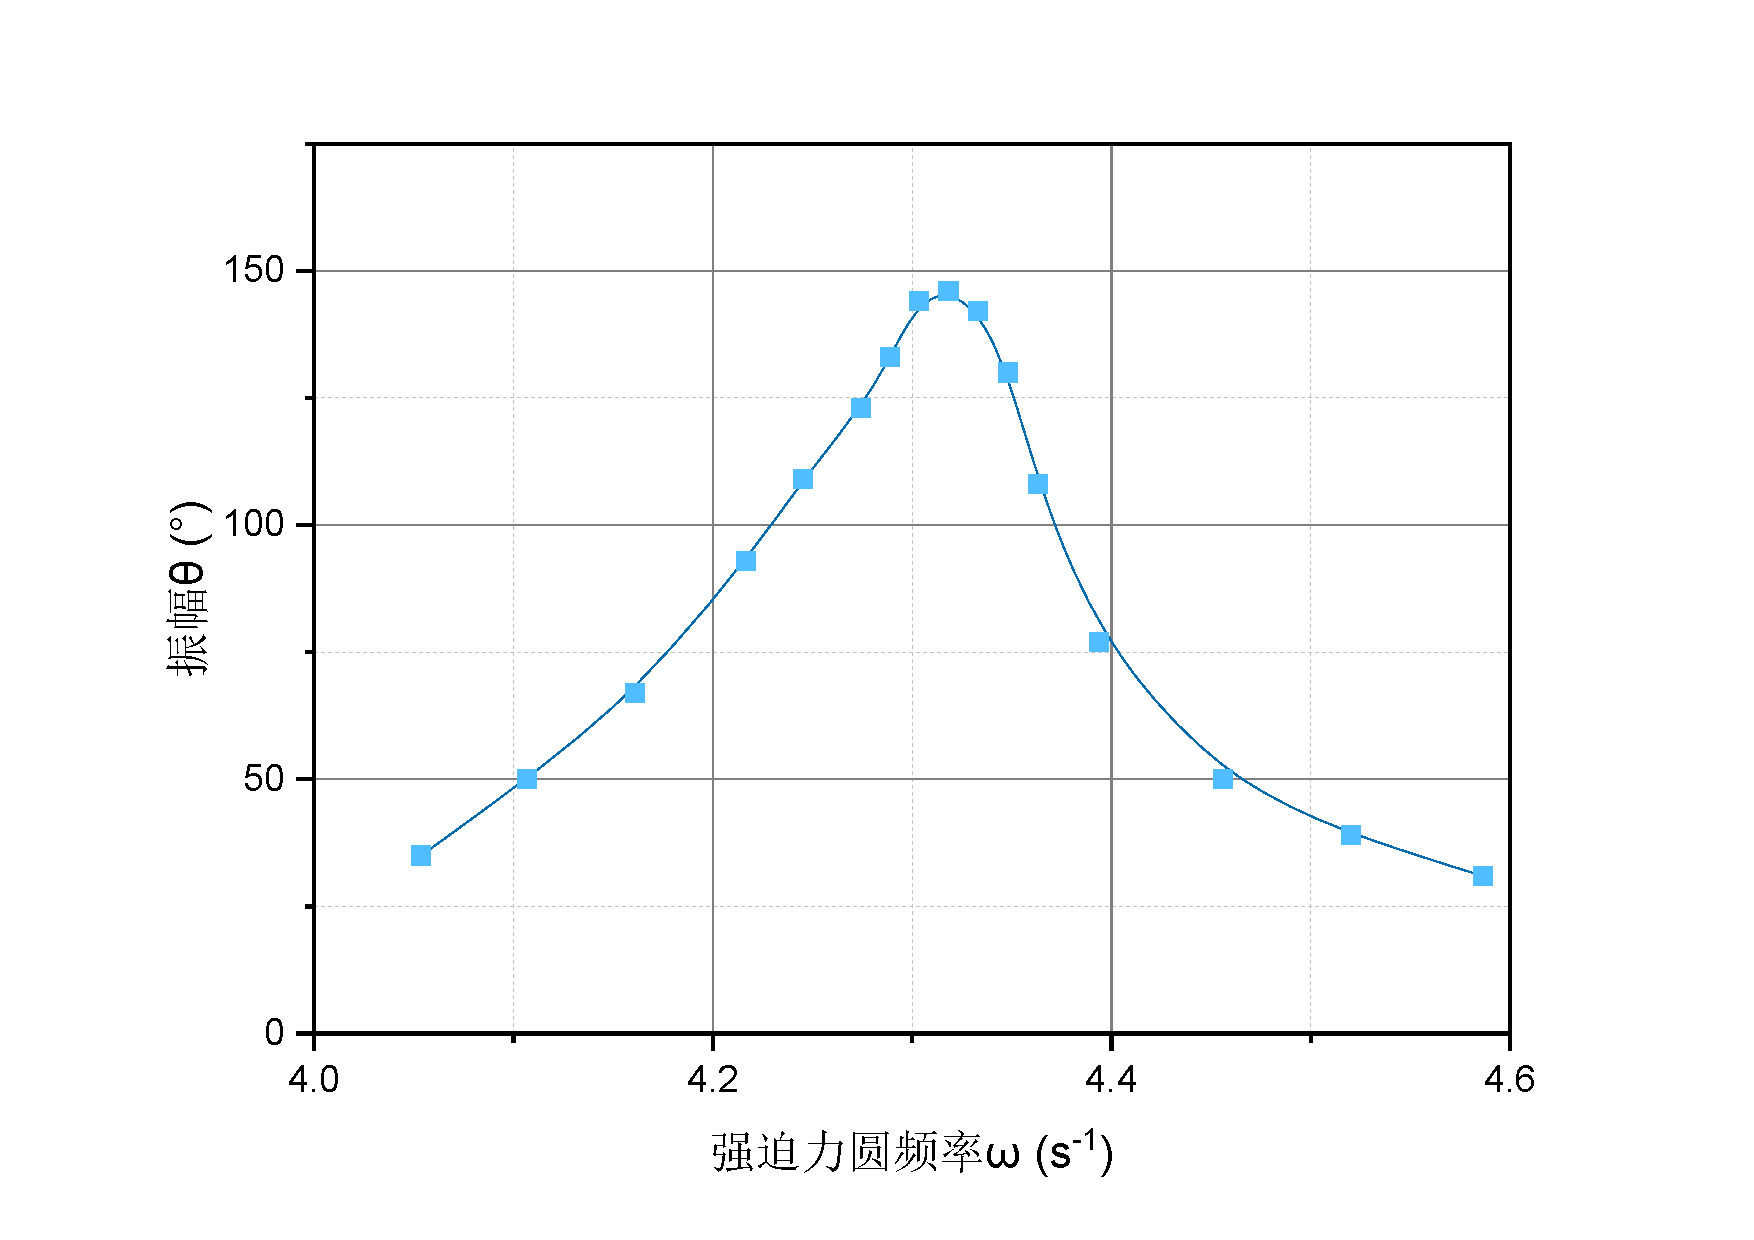
\includegraphics[scale=0.4]{2_theta1.pdf}}\hspace{-20mm}
\subfigure[阻尼2档下相频特性曲线]{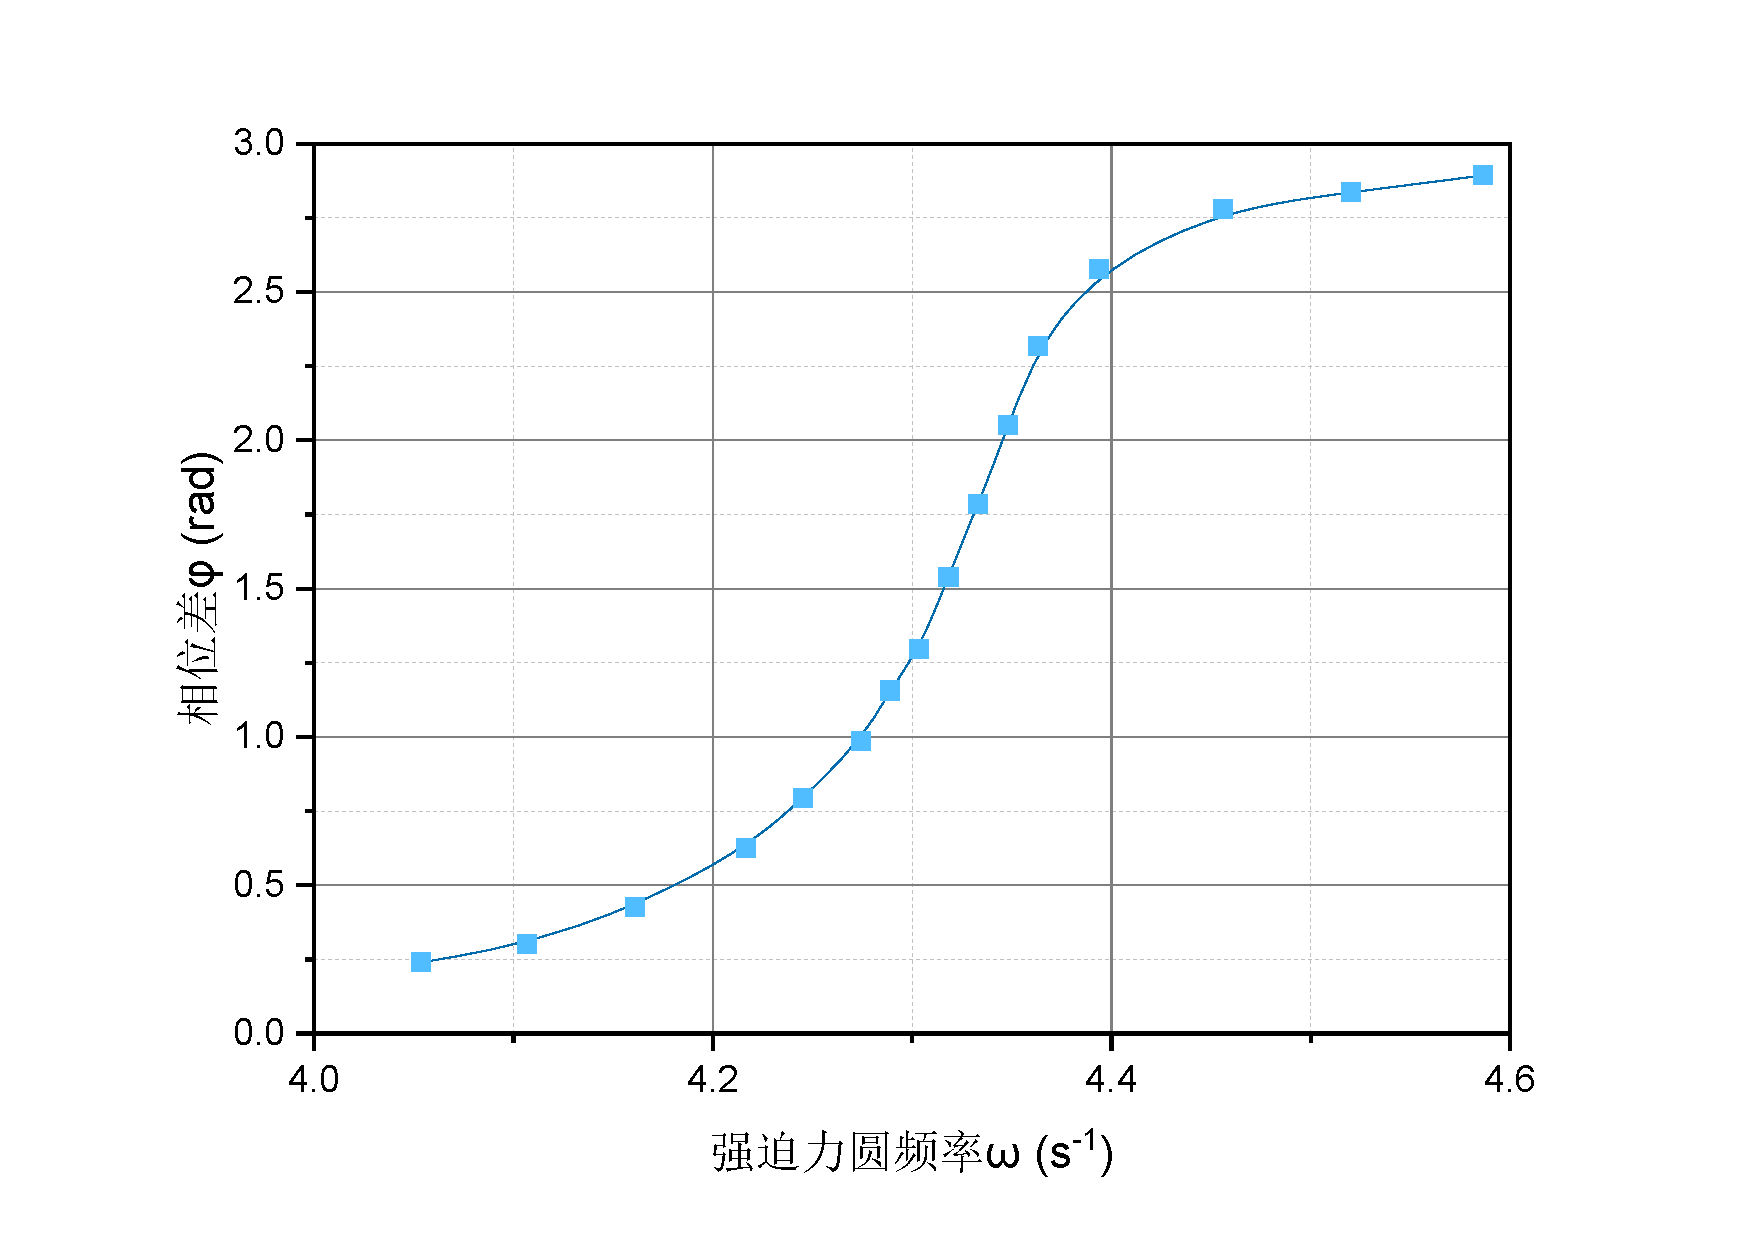
\includegraphics[scale=0.4]{2_phi.pdf}}
\caption{阻尼2档幅频、相频特性曲线}
\restoregeometry
}
\end{figure}

\paragraph{对阻尼3档的数据测量及分析如下:}\quad \par
阻尼二档下测量的数据如下表所示,据此可以画出阻尼2档下的幅频特性曲线和相频特性曲线. 这里利用OriginPro程序,在作出散点图后,用B-spline算法对散点间的连线进行平滑化处理,得到平滑曲线.\par
\begin{table}[H]{\begin{center}\caption{阻尼3档不同强迫力频率下受迫振动数据记录表}%\resizebox{\textwidth}{!}{
\begin{tabular}[H]{|c|c|c|c|c|c|c|c|c|}
\hline
次数&1&2&3&4&5&6&7&8\\
\hline
强迫力周期$T_F/s$&1.372&1.402&1.422&1.432&1.442&1.447&1.452&1.457\\
\hline
强迫力频率$\omega_F/s^{-1}$&4.580&4.482&4.419&4.388&4.357&4.342&4.327&4.312\\
\hline
摆轮振幅$\theta$/°&27&40&60&68&83&94&100&106\\
\hline
相位差1$\phi_1$/°&161.0&154.0&145.0&136.0&123.8&116.0&105.5&94.0\\
\hline
相位差2$\phi_2$/°&164.0&155.5&146.8&137.5&125.0&117.0&106.5&94.5\\
\hline
平均相位差$\phi$/°&162.5&154.8&145.9&136.8&124.4&116.5&106.0&94.3\\
\hline
平均相位差$\phi$/rad&2.836&2.701&2.546&2.387&2.171&2.033&1.850&1.645\\
\hline
次数&9&10&11&12&13&14&15&16\\
\hline
强迫力周期$T_F/s$&1.462&1.467&1.472&1.482&1.492&1.512&1.532&1.552\\
\hline
强迫力频率$\omega_F/s^{-1}$&4.298&4.283&4.268&4.240&4.211&4.156&4.101&4.048\\
\hline
摆轮振幅$\theta$/°&106&104&98&87&78&61&47&34\\
\hline
相位差1$\phi_1$/°&86.5&78.0&68.0&54.0&46.0&30.0&22.0&16.0\\
\hline
相位差2$\phi_2$/°&88.0&79.0&69.5&55.0&47.5&31.5&24.5&18.5\\
\hline
平均相位差$\phi$/°&87.3&78.5&68.8&54.5&46.8&30.8&23.3&17.3\\
\hline
平均相位差$\phi$/rad&1.523&1.370&1.200&0.951&0.816&0.537&0.406&0.301\\
\hline
\end{tabular}%}
\end{center}}\end{table}




\begin{figure}[H]\centering
{
\newgeometry{a4paper,left=0cm,right=1cm}\hspace{-20mm}
\subfigure[阻尼3档下幅频特性曲线]{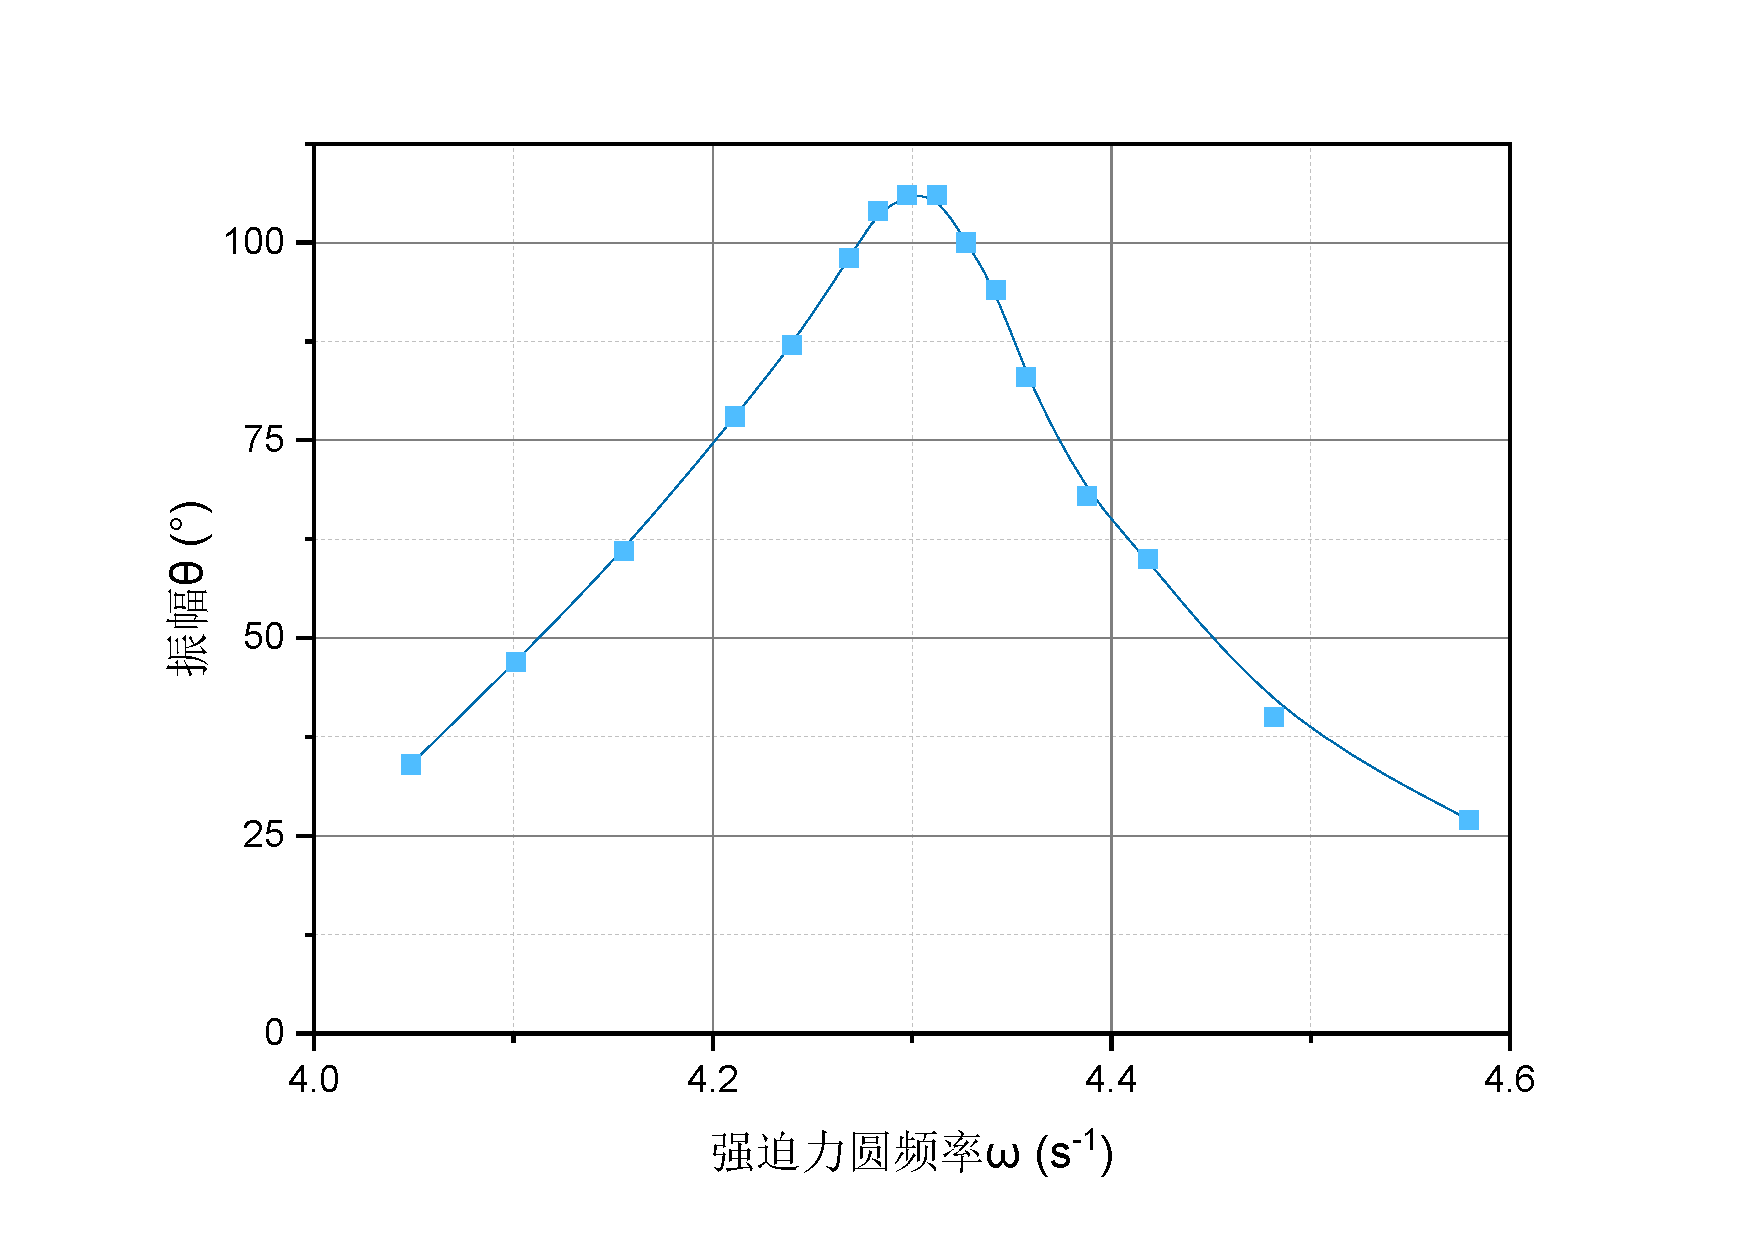
\includegraphics[scale=0.4]{3_theta1.pdf}}\hspace{-20mm}
\subfigure[阻尼3档下相频特性曲线]{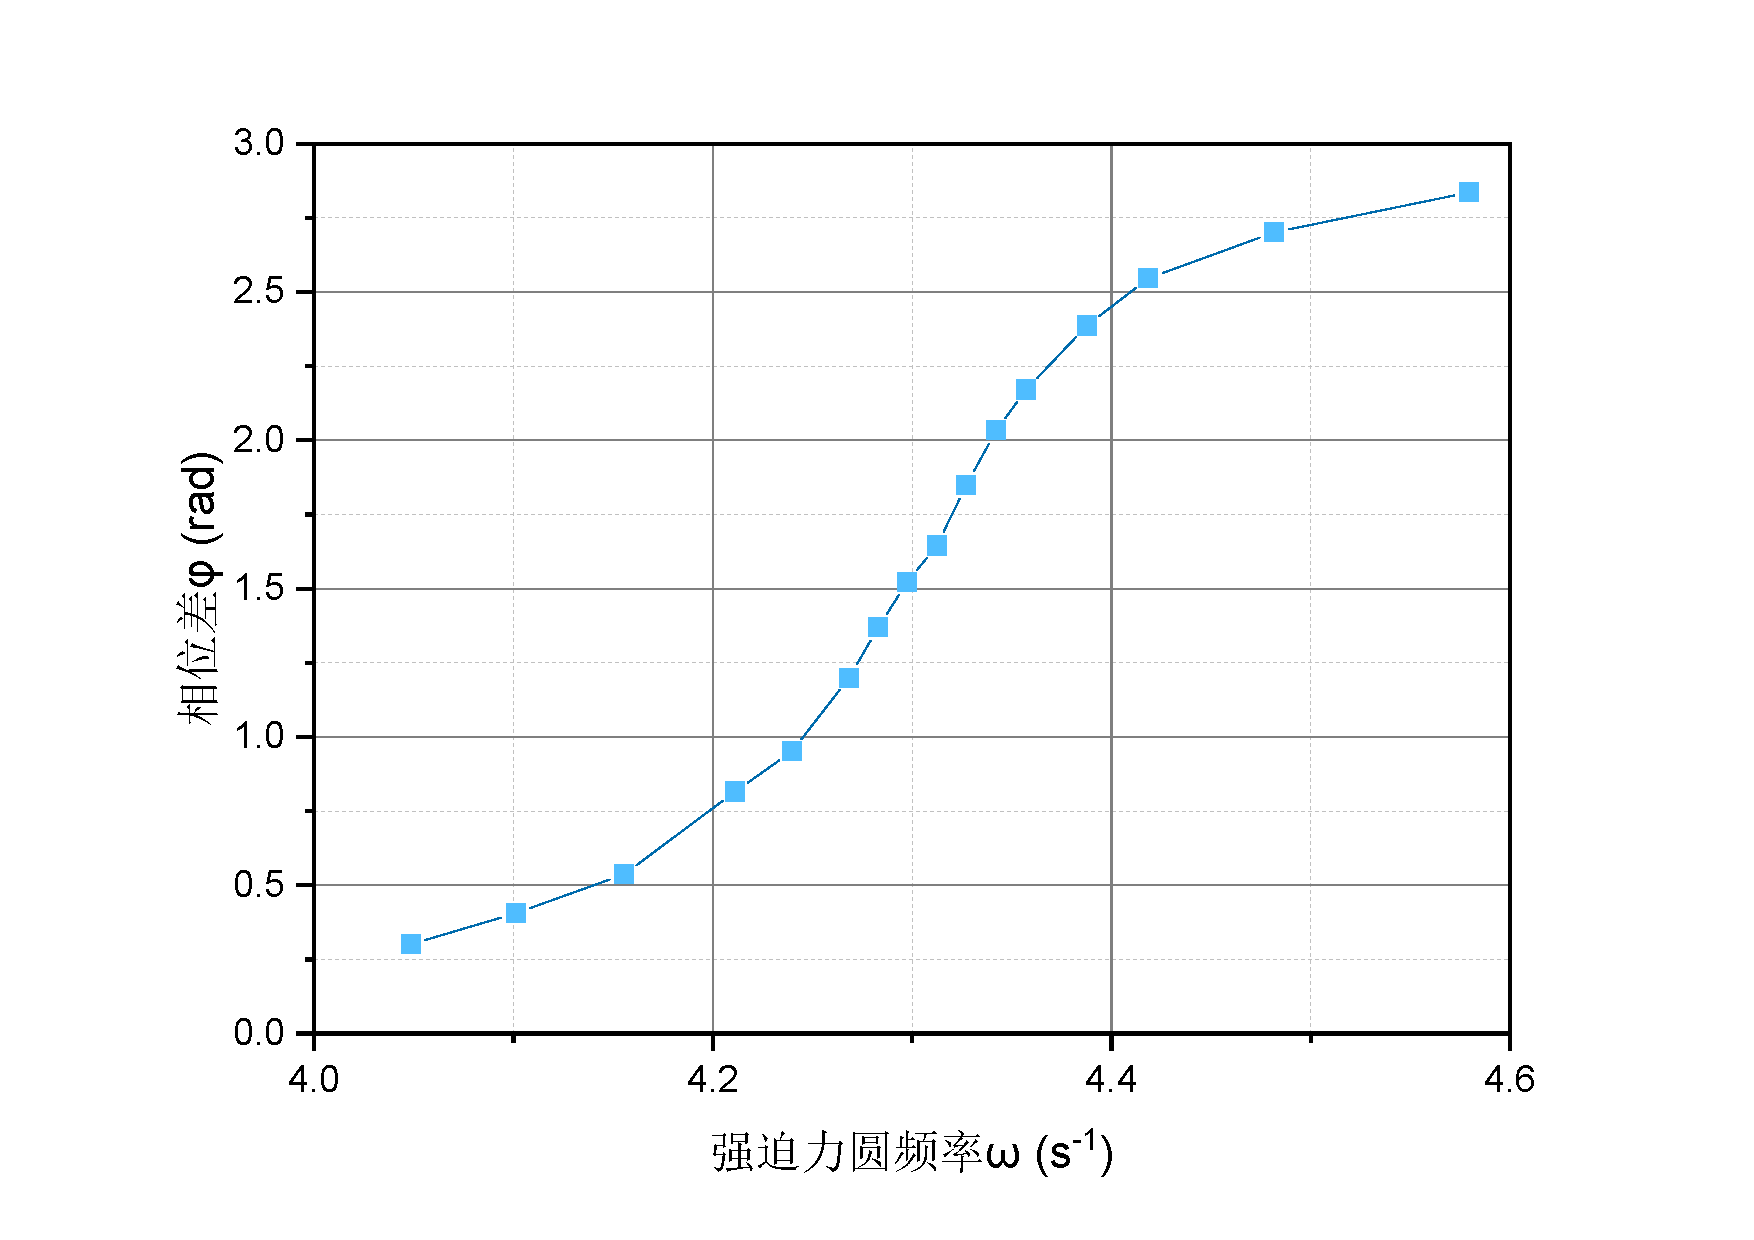
\includegraphics[scale=0.4]{3_phi.pdf}}
\caption{阻尼3档幅频、相频特性曲线}
\restoregeometry
}
\end{figure}

\subsubsection*{B.4 两个幅频特性和相频特性的比较}
下面,将B.3获得的两组幅频、相频特性分别合成在一张图中,如下图所示:
\begin{figure}[H]\centering
{
\newgeometry{a4paper,left=0cm,right=1.5cm}\hspace{-25mm}
\subfigure[幅频特性曲线]{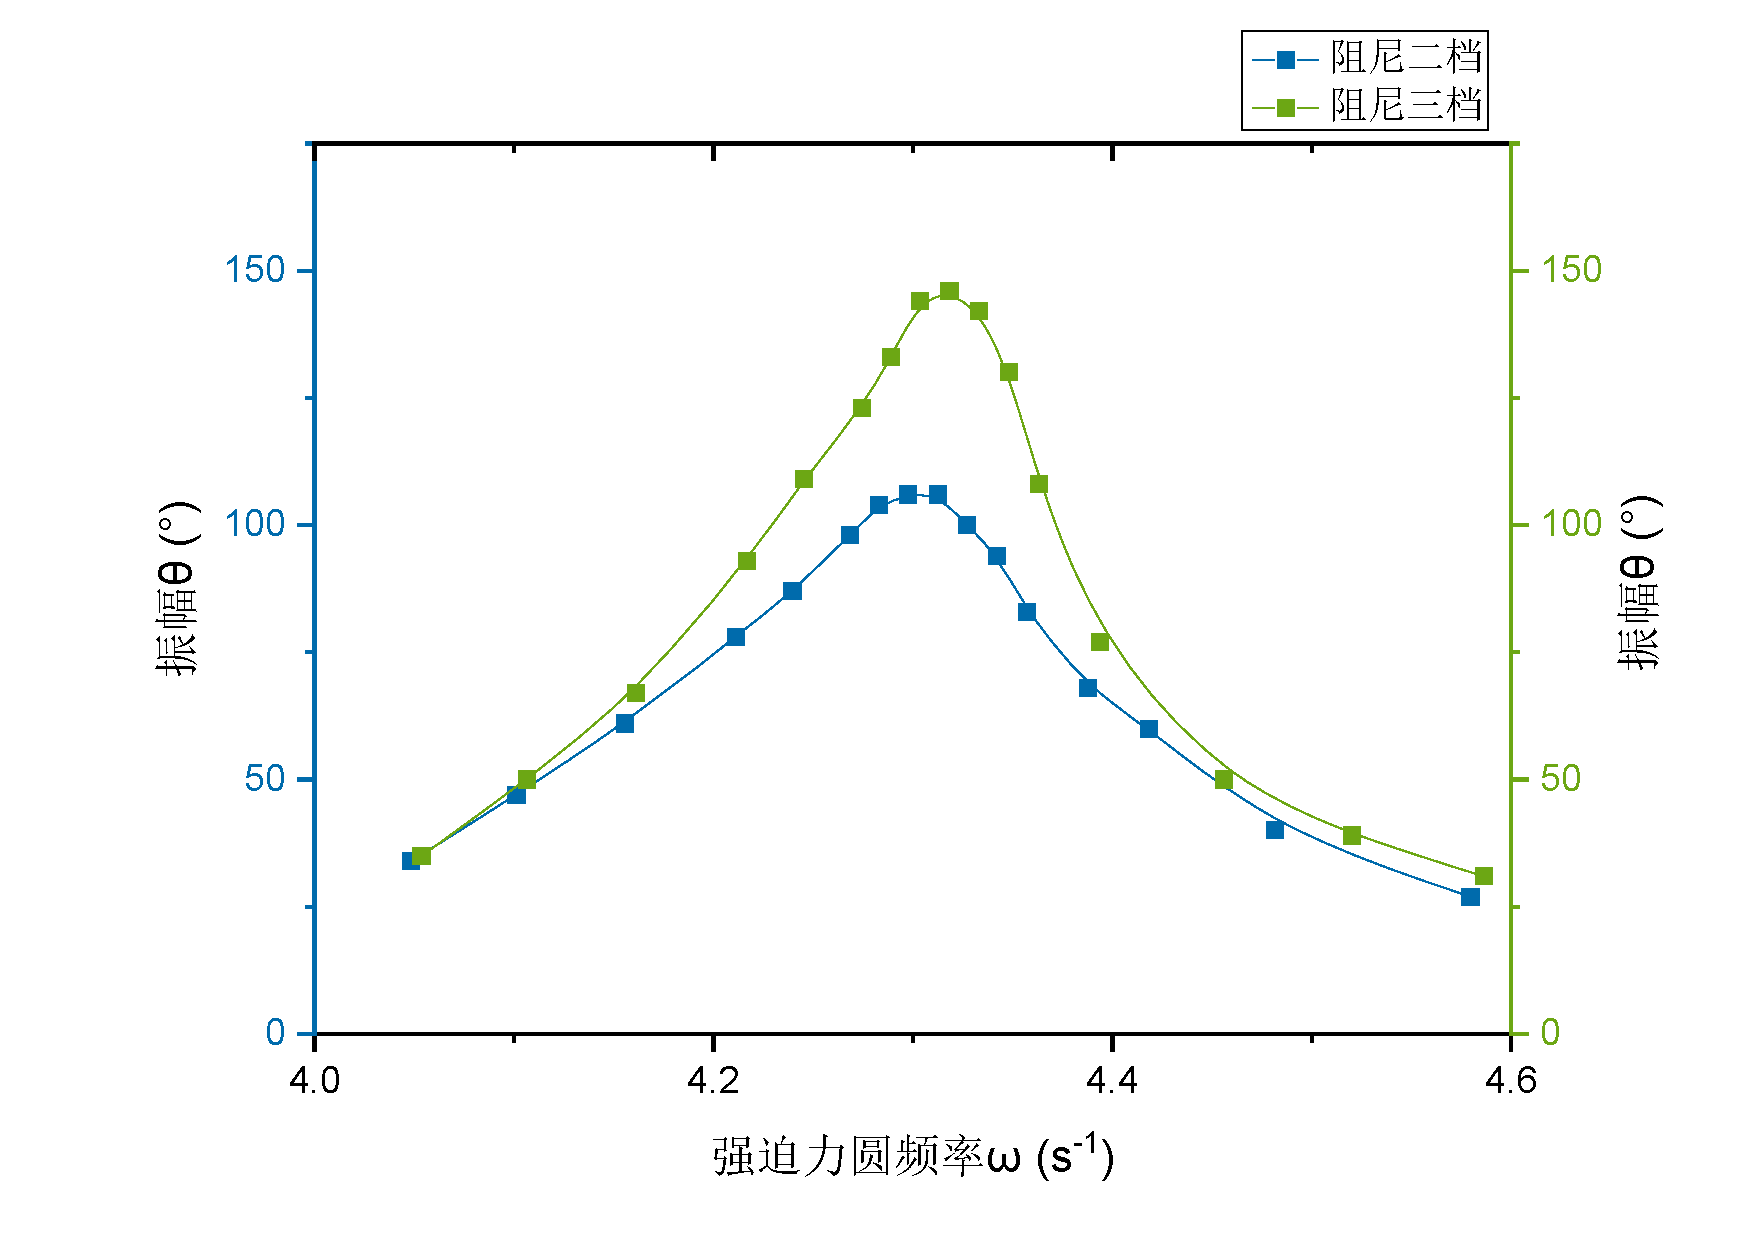
\includegraphics[scale=0.4]{23_theta1.pdf}}\hspace{-15mm}
\subfigure[相频特性曲线]{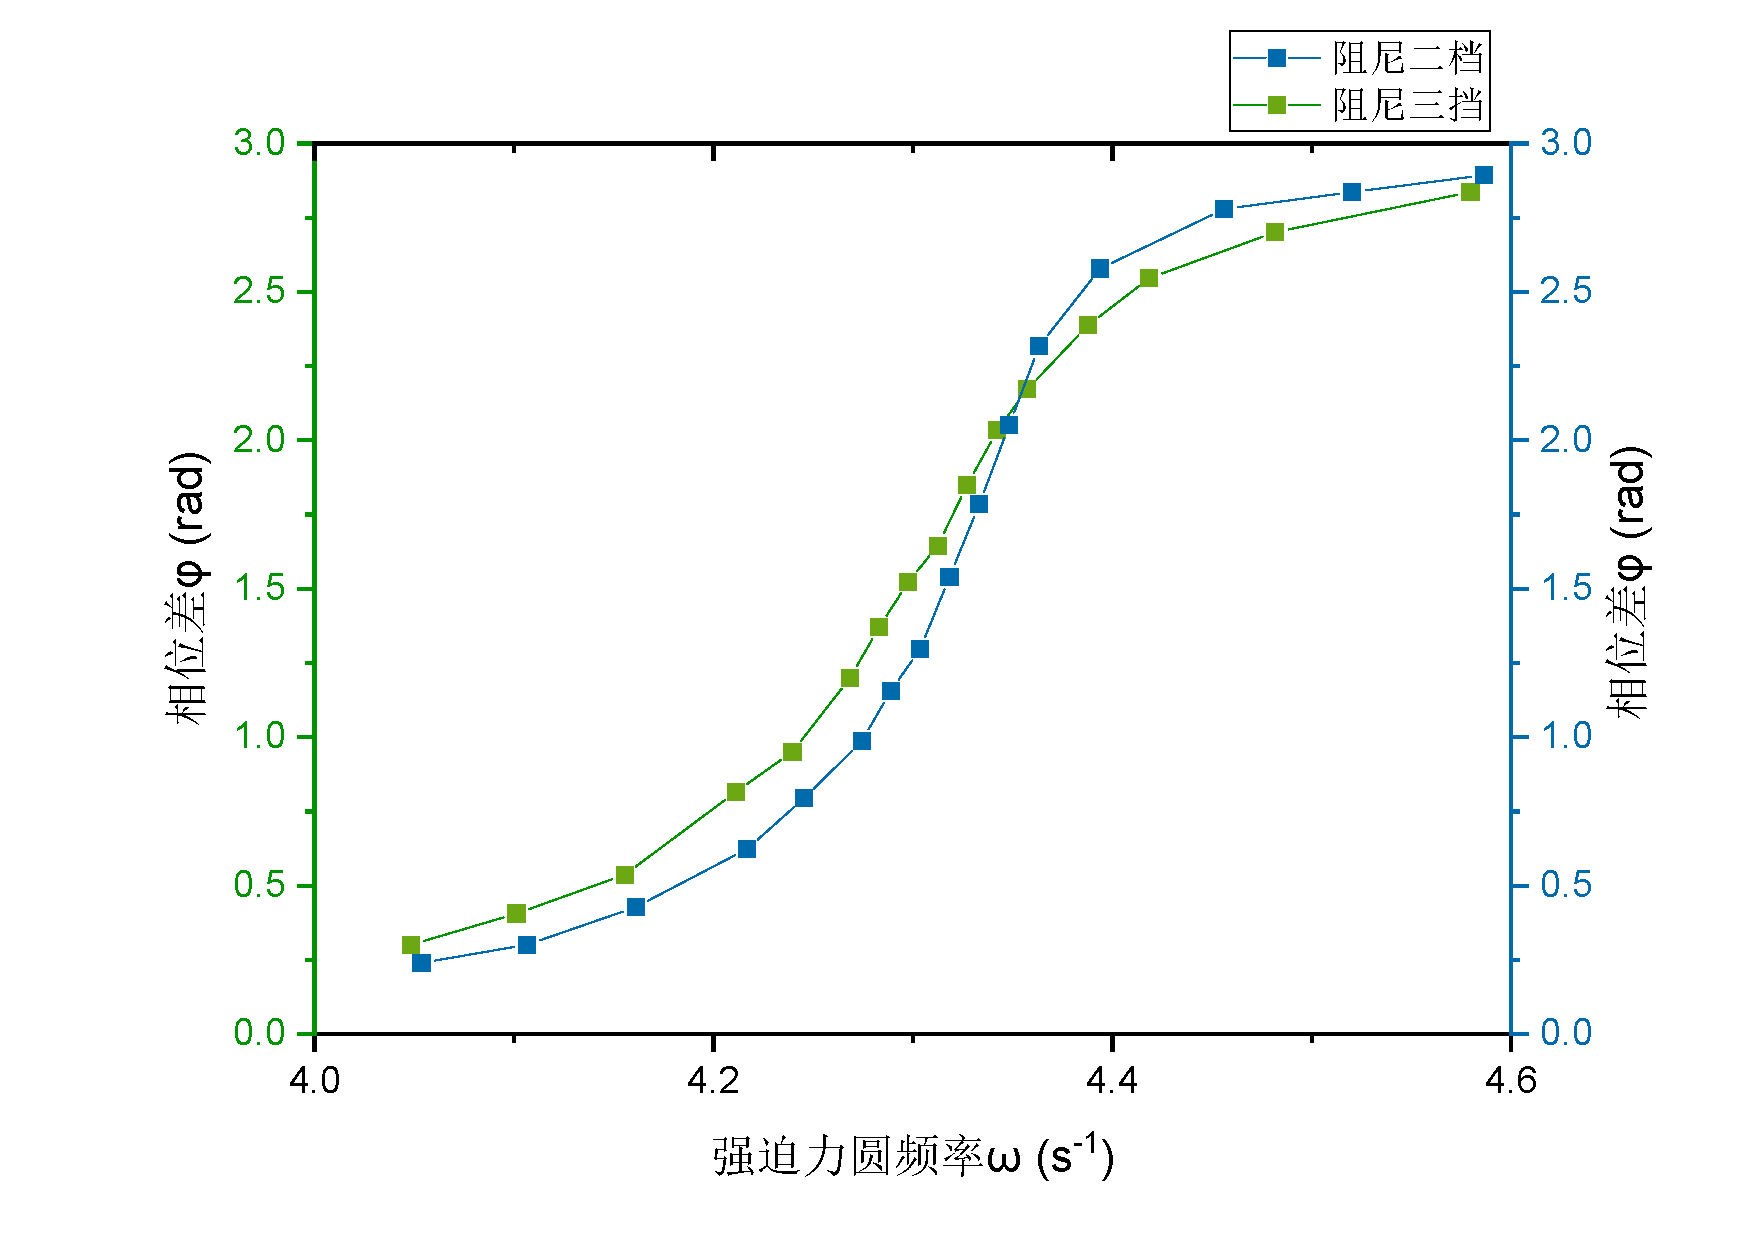
\includegraphics[scale=0.4]{23_phi1.pdf}}
\caption{阻尼2、3档幅频、相频特性曲线}
\restoregeometry
}
\end{figure}
但这里会出现一个问题,即两种阻尼档下共振频率不一样,出现峰值的横轴坐标不同. 对于幅频特性曲线来说,这意味着最大值点不在同一竖直线上;对于相频特性曲线来说,这意味着二者没有共振时相位差为$\frac{\pi}{2}$的交点,这无疑会对图像的特性的把握产生干扰,也破坏了图像本身的对称性. 下面我们可以归一横坐标,即用$\omega/\omega_{res}$的值作为横坐标,以此解决以上两个问题,并对图像的特征进行分析.
\begin{figure}[H]\centering
{
\newgeometry{a4paper,left=0cm,right=1.5cm}\hspace{-25mm}
\subfigure[横坐标归一的幅频特性曲线]{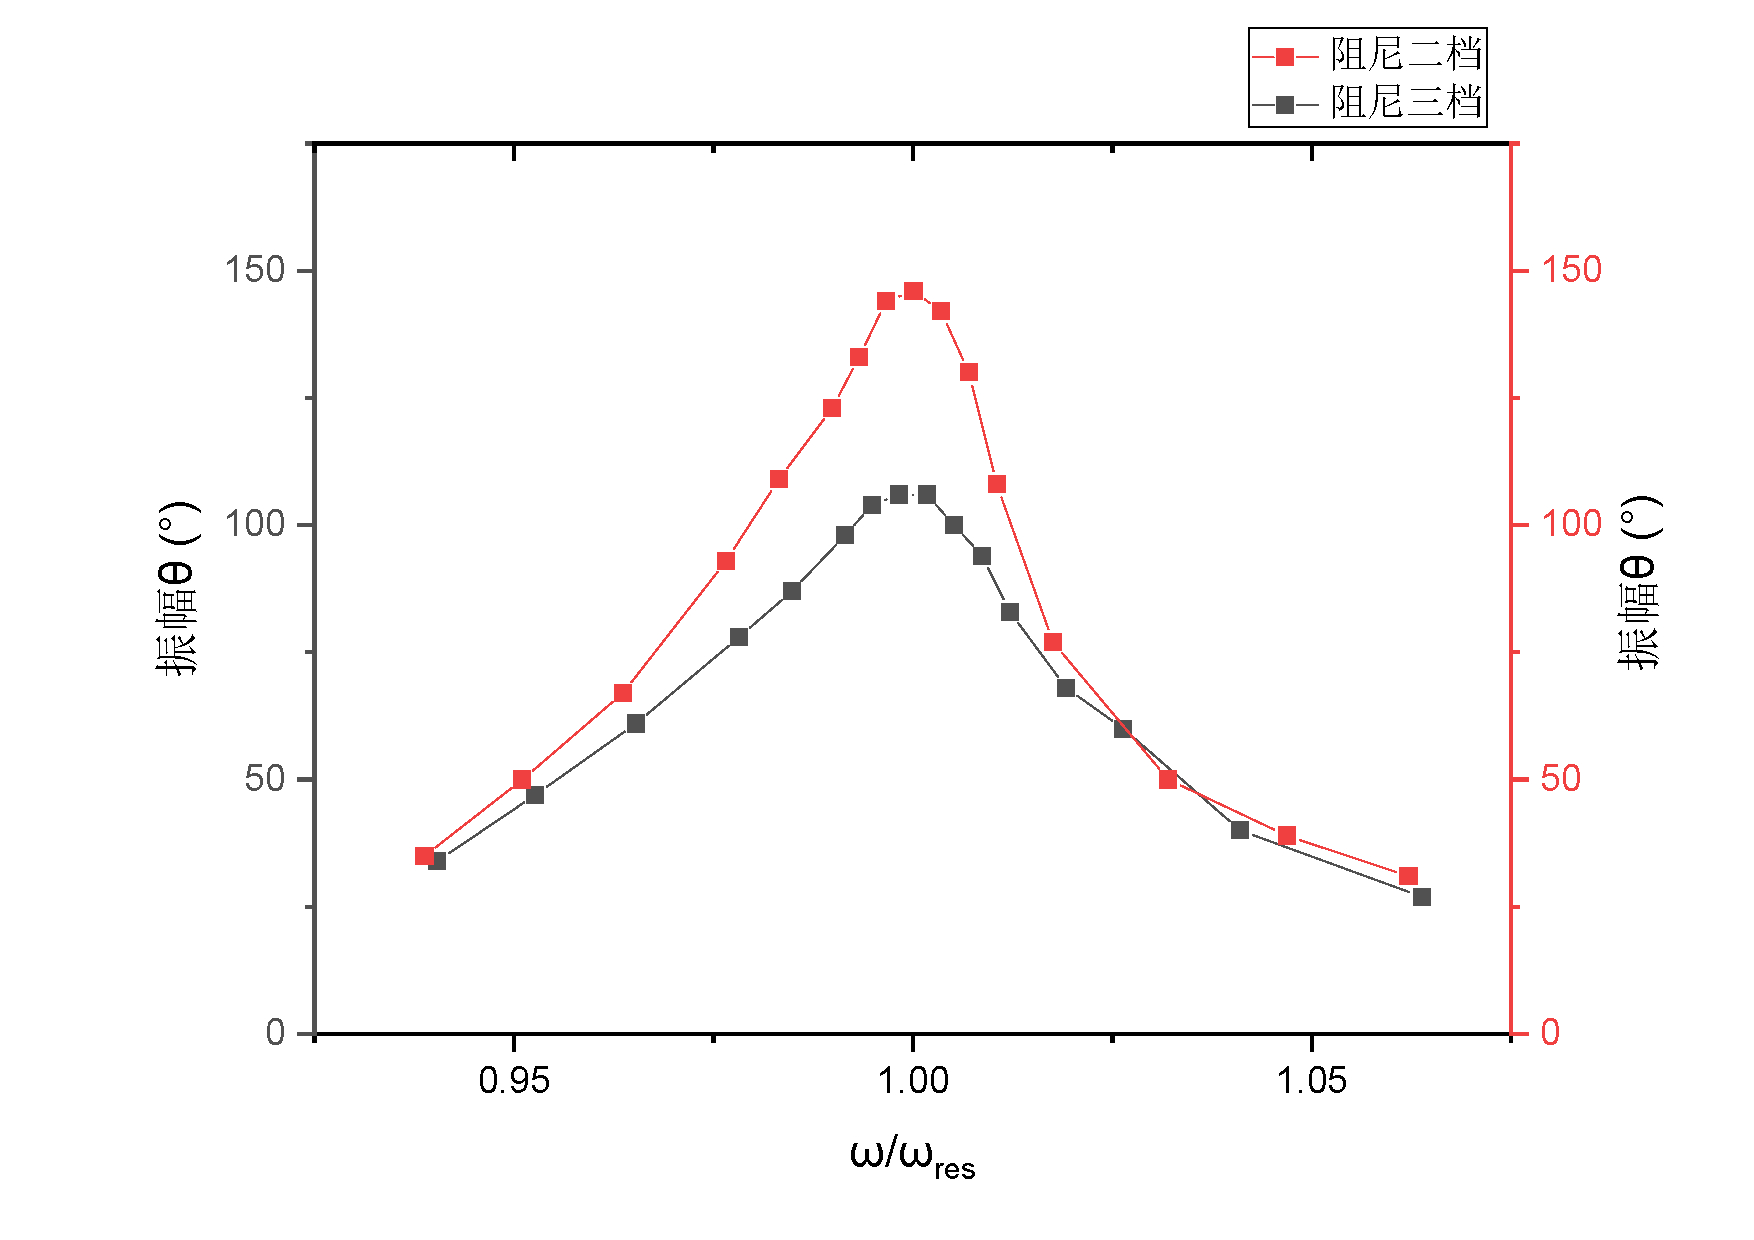
\includegraphics[scale=0.4]{23_theta2.pdf}}\hspace{-15mm}
\subfigure[横坐标归一的相频特性曲线]{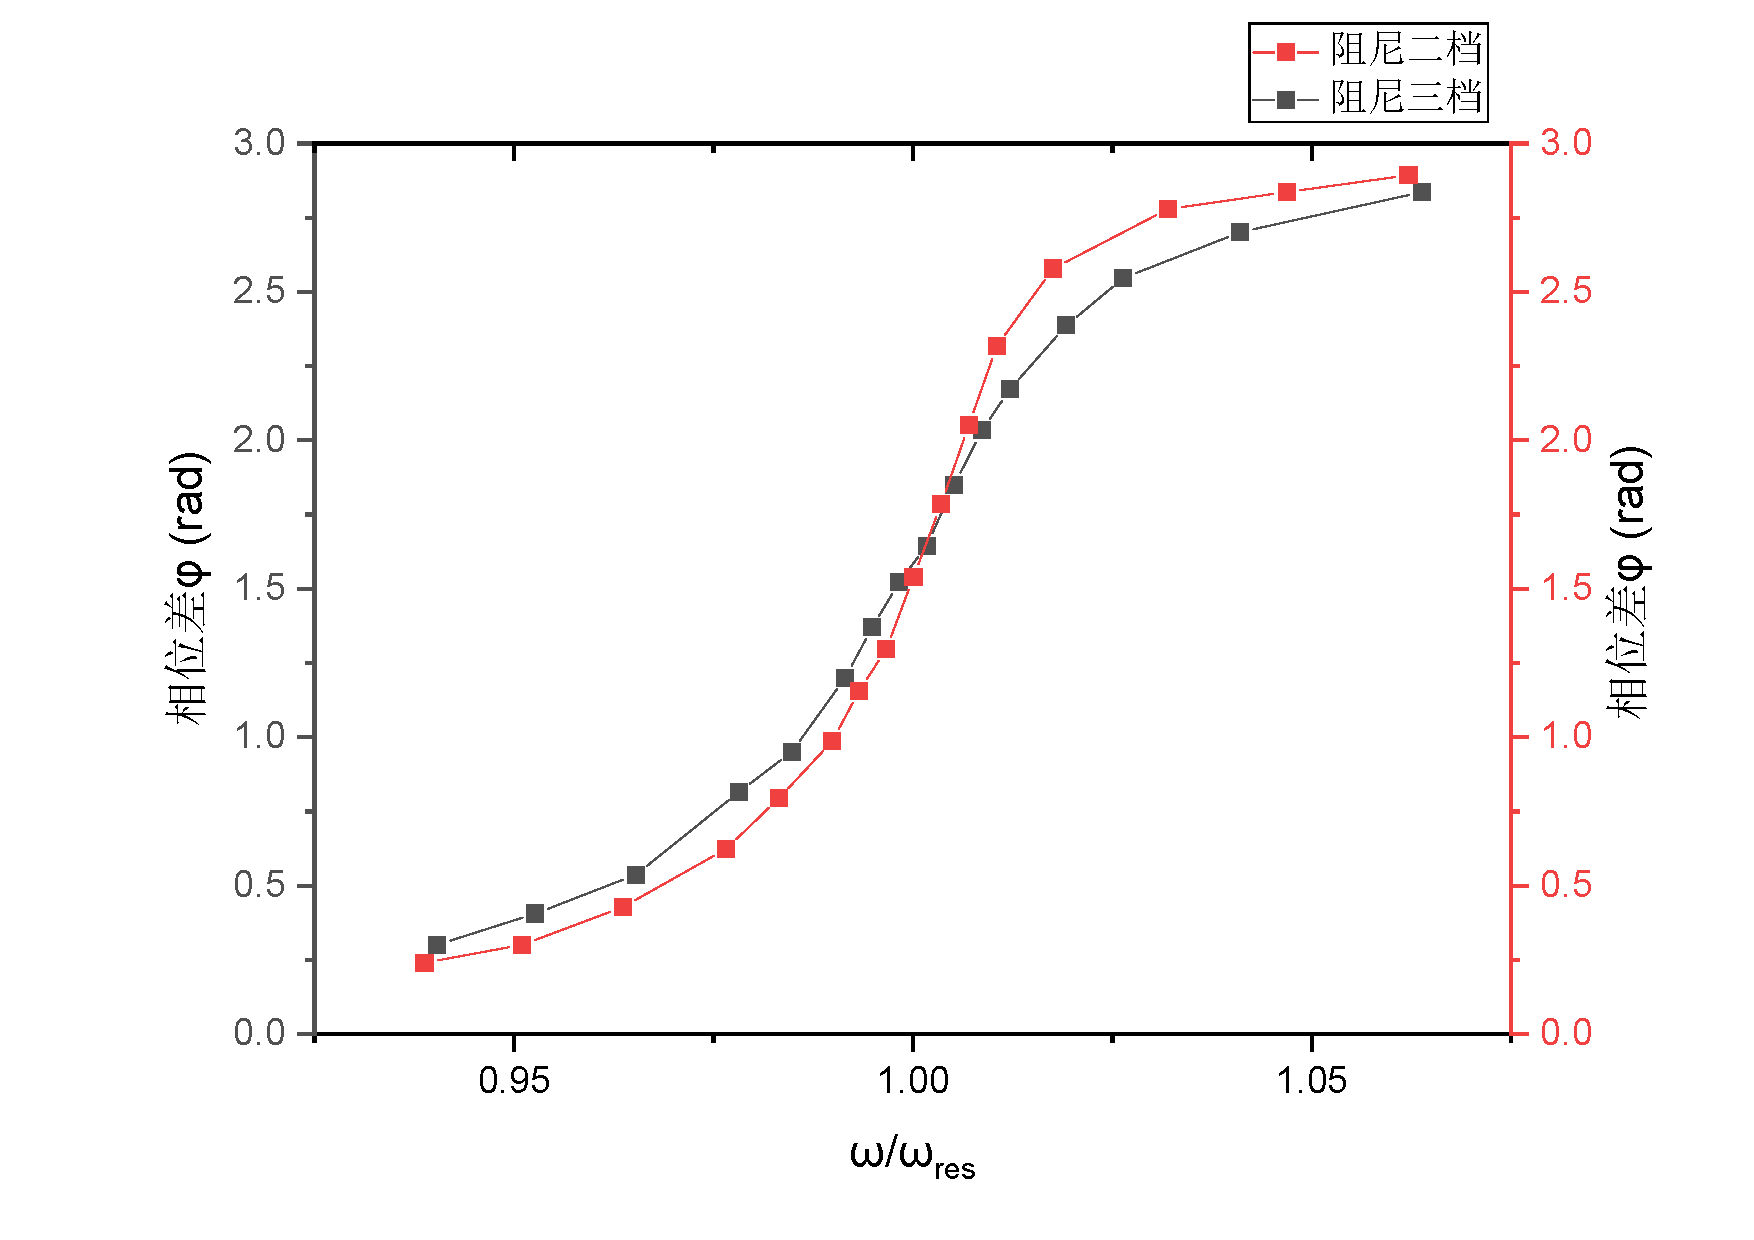
\includegraphics[scale=0.4]{23_phi2.pdf}}
\caption{阻尼2、3档横坐标归一的幅频、相频特性曲线}
\restoregeometry
}
\end{figure}\par
我们首先对幅频特性曲线进行分析. 容易看出,阻尼2档峰值高于3档,这一点与理论相符合. 设$x=\omega/\omega_{res}\approx\omega/\omega_{0}$. 由(\ref{theta})式$\displaystyle{\theta_m=\frac{\omega_0^2A_D}{\sqrt{(\omega_0^2-\omega^2)^2+(2\beta\omega)^2}}=\frac{A_D}{\sqrt{x^4-2x^2+1+\frac{4\beta^2}{\omega_0^2}x^2}}}$,$\beta$减小,$\theta_m$增大.\par
再对相频特性曲线分析,我们容易发现两条曲线大致交于(1,$\frac{\pi}{2}$)点处,而这恰是共振点,说明实验数据与理论相符合. 由(\ref{phi})式,$\displaystyle{\phi=\arctan\frac{2\beta\omega}{\omega_0^2-\omega^2}}$,对$x$求导后发现,$\beta$小时变化率大,这也与图像展示出来的特性相符.
%%%%%%%%%%%%%%%%%%%%%%%%%%%%%%%%%%%%
\subsubsection*{B.5 由幅频特性曲线计算品质因数$Q$}
下面我们讨论幅频特性曲线,由(\ref{theta})式得,令$\theta=\theta_m/\sqrt2$,考虑到对应频率与共振频率相比变化量是个小量,故可记对应点为$\omega_0-\Delta\omega$、$\omega_0+\Delta\omega$,并进行小量近似,可以推导出
\begin{equation}
4\omega_0^2\Delta\omega^2+4\beta^2\omega_0^2=8\beta^2\omega_0^2
\end{equation}
解得$\Delta\omega=\beta$,再由(\ref{Q})式,
\begin{equation}\label{Q2}
Q=\frac{\omega_0}{2\Delta\omega}=\frac{\omega_0}{2\beta}=\frac{\omega_0}{\omega_{+}-\omega_{-}}
\end{equation}
则找出对应$\theta_m/\sqrt2$的对应频率即可计算出品质因数$Q$.

\paragraph{对阻尼2档的数据测量及分析如下:}\quad \par

\begin{figure}[H]\centering{
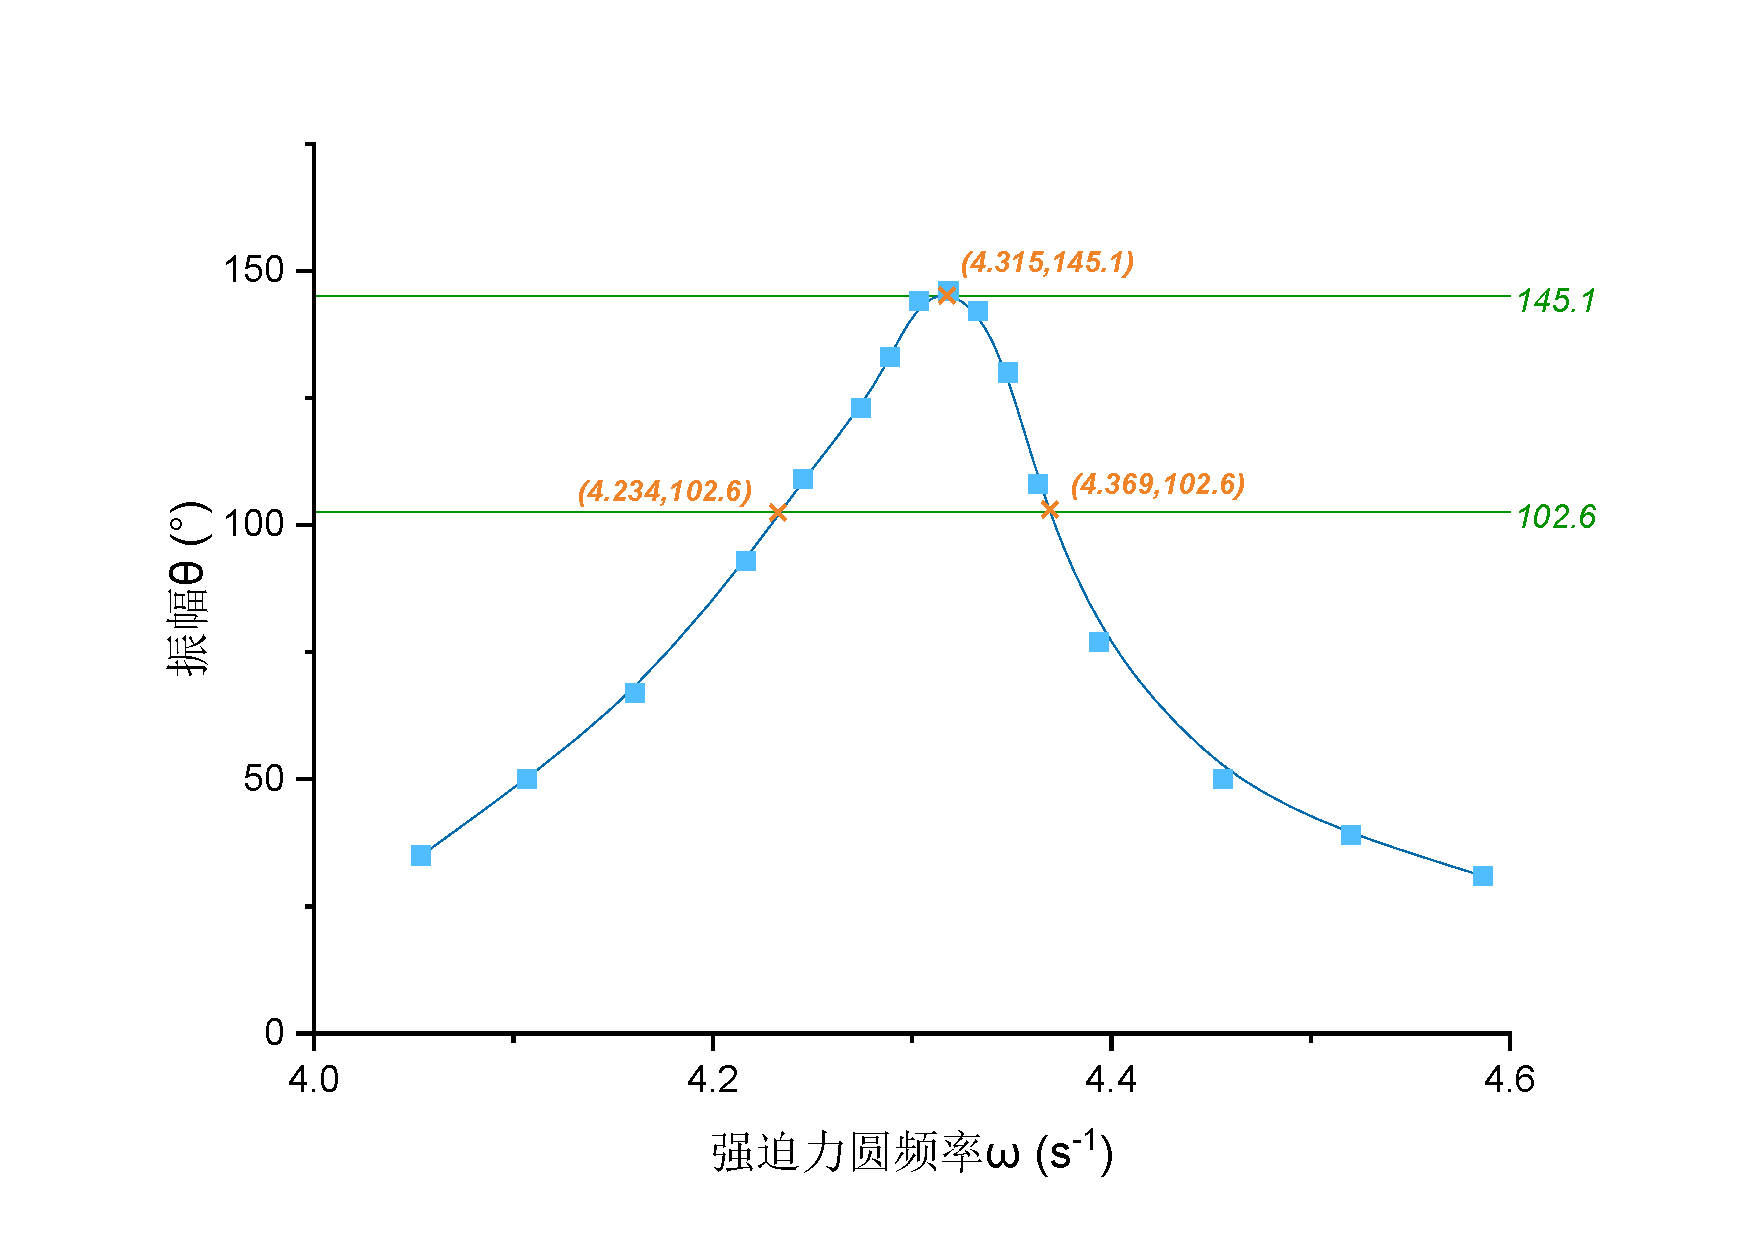
\includegraphics[scale=0.5]{2_theta2.pdf}
\caption{阻尼2档幅频特性曲线}
}\end{figure}

由OriginPro程序,对数据对应的散点图B-spline算法将连线平滑化,作出幅频特性曲线,再利用程序自带的Screen Reader工具,读出最高点对应的坐标为(4.315,145.1),则$\theta_m=145.1$°,那么只需寻找$\theta=\theta_m/\sqrt2=102.6$°对应点. 再利用Screen Reader工具读出直线$\theta=102.6$°与特性曲线的交点为(4.234,102.6)和(4.369,102.6),那么$\omega_{-}=4.234s^{-1}$,$\omega_{+}=4.369s^{-1}$,以此计算出$\displaystyle{Q=\frac{\omega_0}{\omega_{+}-\omega_{-}}=32.0}$,与A.4中计算出的2档品质因数$Q=35.3$接近,数值彼此吻合,验证了实验的正确性.

\paragraph{对阻尼3档的数据测量及分析如下:}\quad \par

\begin{figure}[H]\centering{
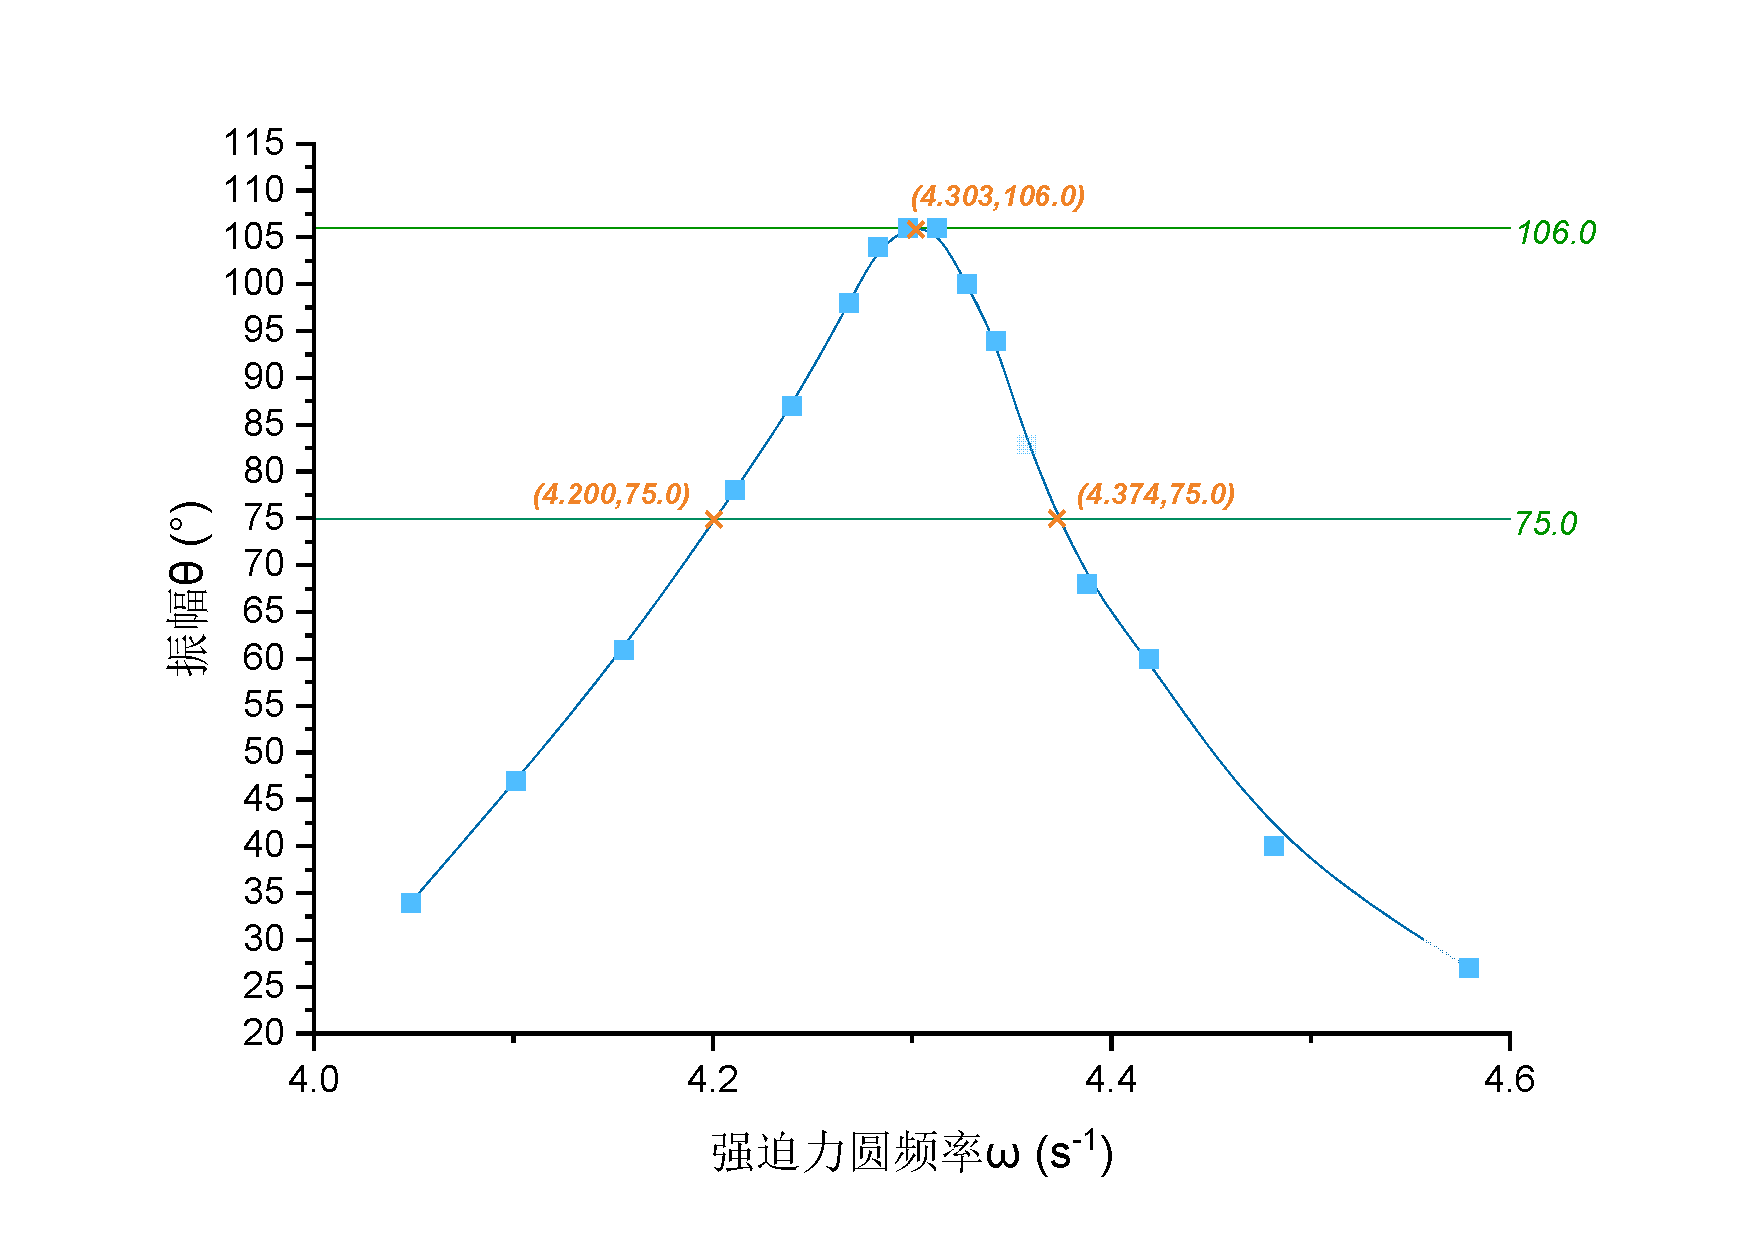
\includegraphics[scale=0.5]{3_theta2.pdf}
\caption{阻尼3档幅频特性曲线}
}\end{figure}

由Originpro程序,对数据对应的散点图B-spline算法将连线平滑化,作出幅频特性曲线,再利用程序自带的Screen Reader工具,读出最高点对应的坐标为(4.303,106.0),则$\theta_m=106.0$°,那么只需寻找$\theta=\theta_m/\sqrt2=75.0$°对应点. 再利用Screen Reader工具读出直线$\theta=75.0$°与特性曲线的交点为(4.200,75.0)和(4.374,75.0),那么$\omega_{-}=4.200s^{-1}$,$\omega_{+}=4.374s^{-1}$,以此计算出$\displaystyle{Q=\frac{\omega_0}{\omega_{+}-\omega_{-}}=24.7}$,与A.4中计算出的2档品质因数$Q=24.2$接近,数值彼此吻合,验证了实验的正确性.

%%%%%%%%%%%%%%%%%%%%%%%%%%%%%%%%%%%%%
\subsection*{ C) 探究受迫振动的瞬态过程}
\subsubsection*{C.1 受迫振动的瞬态过程}
5倍时间常数
研究强迫力为共振频率下的暂态过程,为此我们将阻尼档打至3档,强迫力周期调至B.3测量出的振幅最大值附近作为共振频率对应的周期. 考虑到此实验仪器本身对周期的测量误差限达到$0.002s$,因此取B.3得到的共振频率数据作为近似是合理的. 我们取$T_F=1.460s$作为强迫力周期,共振频率大约为$\omega_d=\omega_0=4.318s^{-1}$.\par
\paragraph{对瞬态过程进行定性观察}\quad\par
使摆轮处于静止的状态,打开电机,发现振幅是逐渐增大而不是直接达到稳态的. 下面我们对这一现象进行理论分析.\par
首先欠阻尼条件下下可以认为$\displaystyle{\sqrt{\omega_0^2-\beta^2}\approx\omega\approx\omega_0}$. 由(\ref{tongjie})式,欠阻尼条件下运动方程为\\$\displaystyle{\theta=\theta_0e^{-\beta t}\cos(\sqrt{\omega_0^2-\beta^2}t+\phi_0)+\theta_m\cos(\omega t-\phi)}$. 由(\ref{phi})式,共振时$\phi=\frac{\pi}{2}$. 再由约束条件$\theta=0$得:$\phi_0=\pm \frac{\pi}{2}$. 由约束条件$\dot{\theta}=0$,可以得到$\phi_0=\frac{\pi}{2}$,且可以近似得到$\theta_0\approx \theta_m$,则运动方程可改写为:
\begin{equation}\label{approx}
\theta=\theta_m(1-e^{-\beta t})sin(\omega_0t)
\end{equation}
它是一个由此得到的图像大约如下图所示
\begin{figure}[H]\centering{
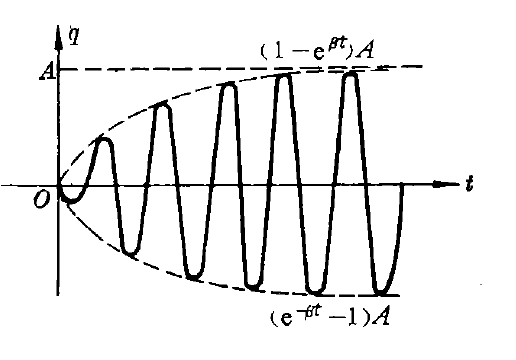
\includegraphics[scale=0.45]{ref.png}
\caption{暂态过程运动示意图}}
\end{figure}
由摆轮幅度是逐渐加大的.

\paragraph{对瞬态过程进行数据记录}\quad\par
关闭电机,待摆轮停止后在开动电机,对摆轮每一周期的振动幅度进行测量. 由B.2判断稳态的方法之估算,我们可以估算$5\tau\approx50s$后达到稳态. 从另一角度,可以根据振幅变化的规律,认定若干周期内振幅不变即达到稳态. 下面是对每周期振幅的测量,测得稳态时振幅为$\theta_m=103$°. 数据如下表:
\begin{table}[H]{\begin{center}\caption{阻尼3档共振频率下摆轮振幅数据记录表}%\resizebox{\textwidth}{!}{
\begin{tabular}[H]{|c|c|c|c|c|c|c|c|c|c|c|}
\hline
周期数$n$&1&2&3&4&5&6&7&8&9&10\\
\hline
振幅$\theta$/°&11&21&30&39&47&53&59&64&69&73\\
\hline
周期数$n$&11&12&13&14&15&16&17&18&19&20\\
\hline
振幅$\theta$/°&76&79&81&84&86&88&89&91&92&93\\
\hline
周期数$n$&21&12&13&14&15&16&17&18&19&20\\
\hline
振幅$\theta$/°&94&95&96&97&97&98&98&99&99&99\\
\hline
周期数$n$&31&32&33&34&35&36&37&38&39&40\\
\hline
振幅$\theta$/°&100&100&101&101&101&101&101&101&101&102\\
\hline
周期数$n$&41&42&43&44&45&46&47&48&49&50\\
\hline
振幅$\theta$/°&102&102&102&102&102&102&102&103&103&103\\
\hline
周期数$n$&51&52&53&54&55&56&57&58&59&60\\
\hline
振幅$\theta$/°&103&103&103&103&103&103&103&103&103&103\\
\hline
\end{tabular}%}
\label{zunisandang}
\end{center}}\end{table}
\paragraph{利用实验数据绘图并与理论图线比较}\quad\par
利用OriginPro制作散点图,并利用B-spline算法对连线平滑化处理,获得振幅随时间变化的实验图线.\par
理论图线可以近似等效为(\ref{approx})式的非振荡项(包络线方程)$\displaystyle{\theta=\theta_m(1-e^{-\beta t})}$. 采用A.3测得的阻尼2档阻尼系数$\beta=0.0894s^{-1}$,并采用本小节前述的$\theta_m=103$°,则函数表达式为$\theta=103(1-e^{-0.0894t})$°.\par
下图将理论图线与实验测得的图线表示在一起以作对比.
\begin{figure}[H]\begin{center}
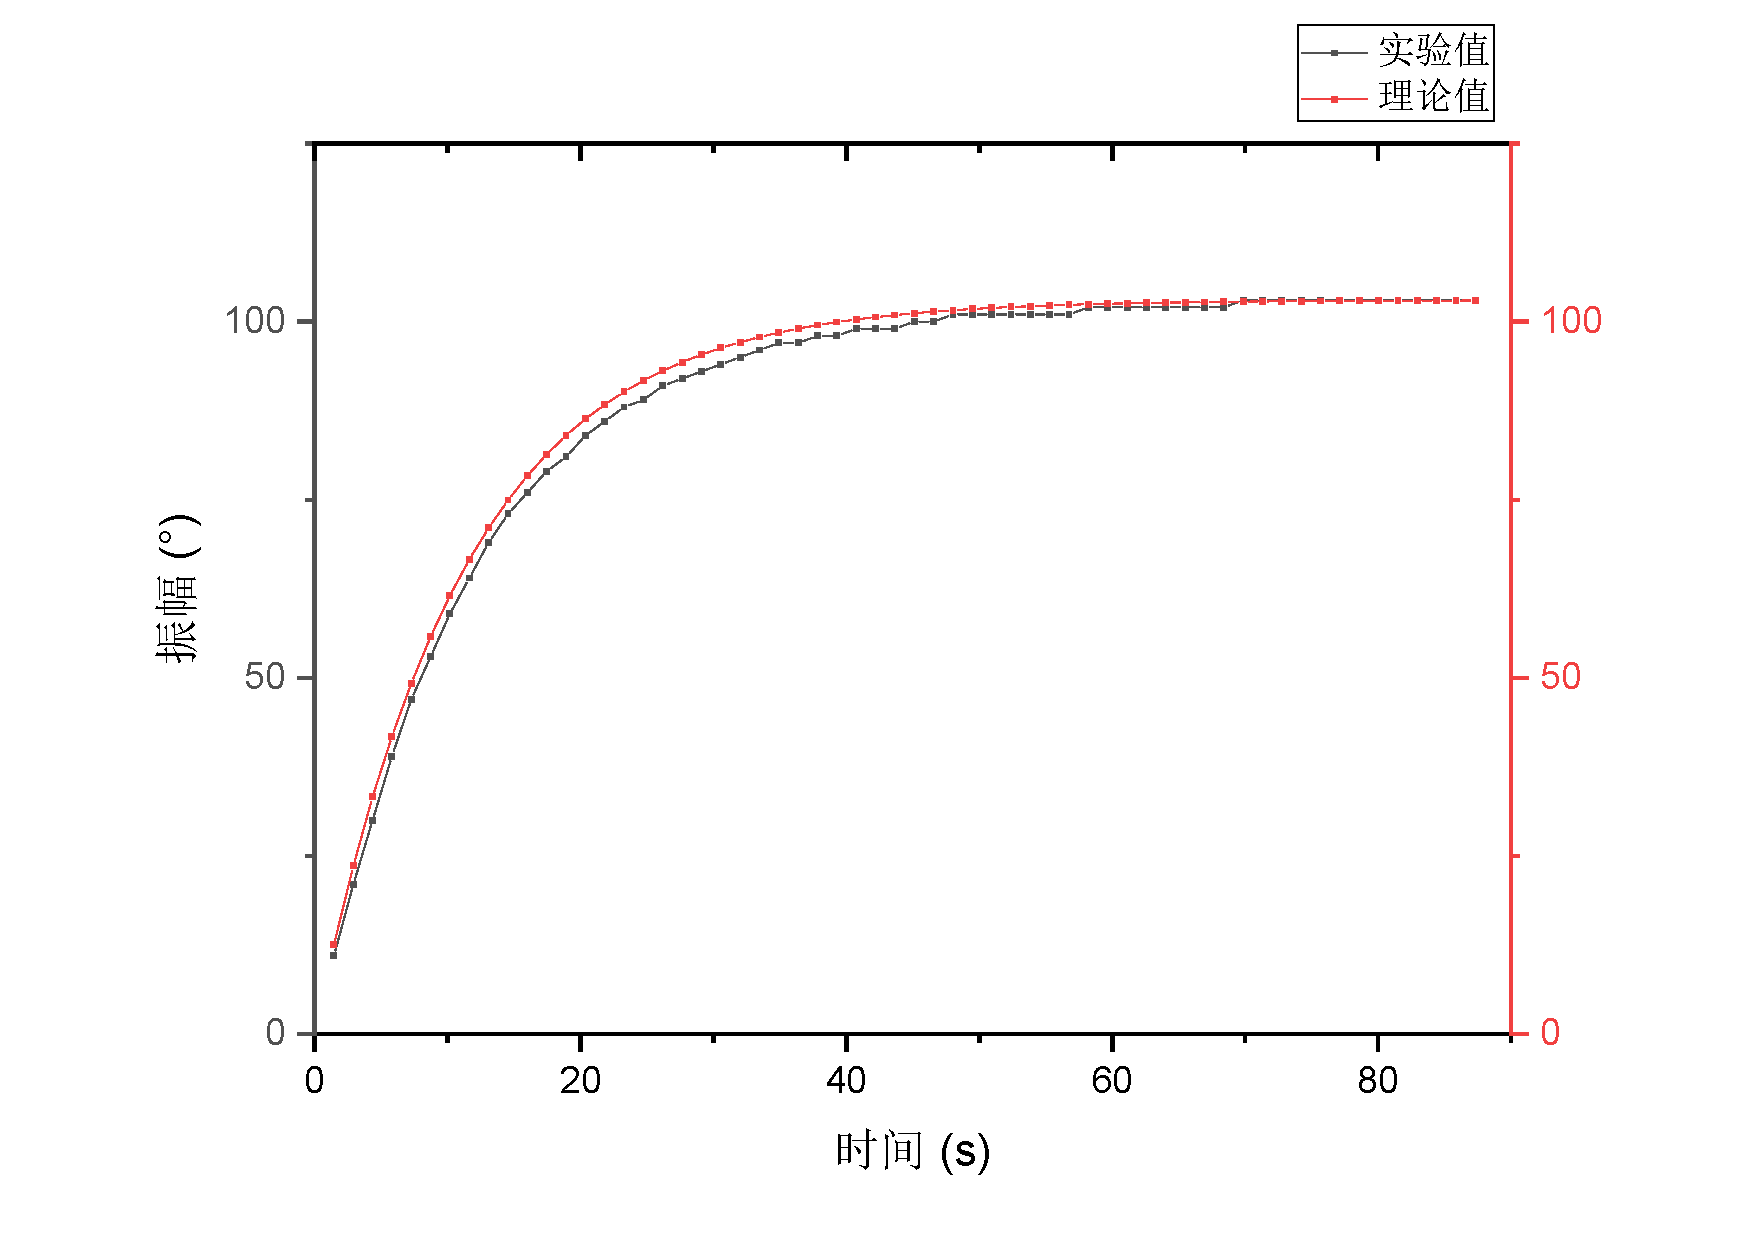
\includegraphics[scale=0.4]{transient.pdf}\vspace{-5mm}
\caption{受迫振动暂态过程实验与理论图线}
\end{center}\end{figure}
可以看出,实验测量与理论吻合较好,验证了理论模型的正确性,也验证了前述测量值的正确性.
同时,我还利用OriginPro的非线性拟合功能,利用模型$y=A(1-e^{-Bx})$对实验数据进行拟合,结果如下:

\begin{figure}[H]\begin{center}
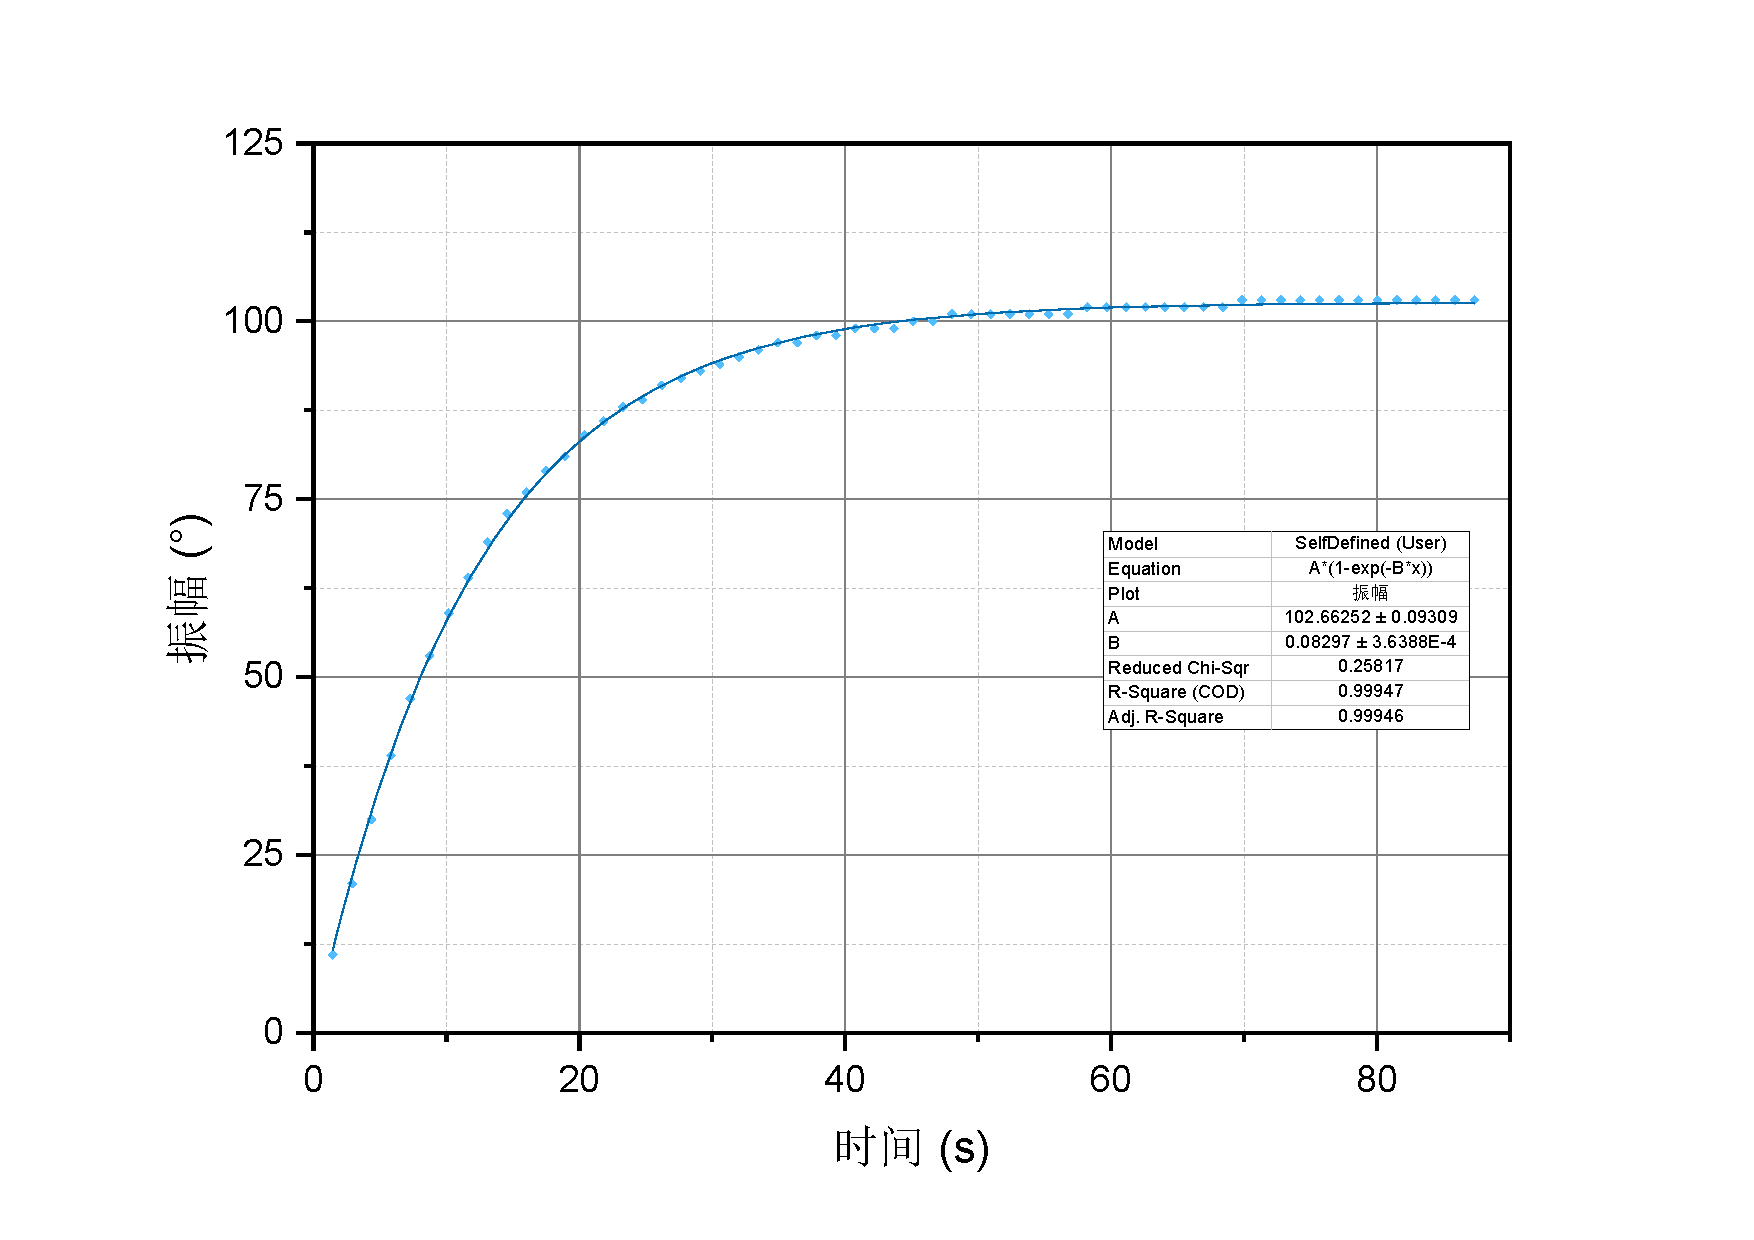
\includegraphics[scale=0.4]{transient_ideal.pdf}\vspace{-5mm}
\caption{受迫振动暂态过程实验数据拟合图线}
\end{center}\end{figure}
可以看出,拟合出$B=0.08927$,与阻尼3档阻尼系数实验值$\beta=0.0894s^{-1}$相近,且该拟合$R^2=0.99946$,接近于1,说明该模型是可靠的.
\subsubsection*{C.2 平均输入功率的计算}
由以上分析,摆轮在共振频率下达到稳态的运动方程为$\theta=\theta_m\cos(\omega_0+\phi)$. 设稳态后体系总能量为$E$,一周期损耗能量为$\Delta E$,电机需要持续提供的平均输入功率为$P$,则有
$\dot{\theta}=-\theta_m\omega_0\sin(\omega_0+\phi)$,平衡位置角速度为$\dot{\theta}_0=\theta_m\omega_0$,那么\\
\[E=\frac{1}{2}I\dot{\theta}_0^2=\frac{1}{2}I\omega_0^2\theta_m^2\textcircled{1}\]
\[\omega_0=\sqrt{\frac{k}{I}}\textcircled{2}\]
\[Q=2\pi\frac{E}{\Delta E}\textcircled{3}\]
\[P=\frac{\Delta E}{T_0}=\frac{\omega\Delta E}{2\pi}\textcircled{4}\]
联立以上\textcircled{1}-\textcircled{4}式得
\begin{equation}
P=\frac{k\omega_0\theta_m^2}{2Q}
\end{equation}
此即稳态后电机提供的平均输入功率表达式.
\section{思考与讨论}
%%%%%%%%%%%%%
\paragraph{1.\quad 对B.2判断稳态方法的补充}\quad\par
我们已在B.2节中提及两种判断受迫振动达到稳态的方法,一者为估算时间常数,一者为观察振幅和相位差,下面我还将提出一种新的思路.\par
实验过程中,我们发现等待足够长时间观察振幅是否改变这一方法缺少可操作性,实验者不知等待的时间,极易造成效率降低抑或没有等到稳态就记录数据. 为此,我将对等待时间进行理论上的估计.
我们对(\ref{approx})的推导过程进行类似的演算,由于测试周期为$0.93T_0-1.07T_0$,据$T_0$相差不大,则有振幅表达式
\begin{equation}
\theta=\theta_m(1-e^{-\beta t})
\end{equation}
实验中,测量的稳态振幅基本在$1\times10^2$°,仪器最小分度值为1°,取$\beta=0.1s^-1$数量级,则$t_{98\%}=-\frac{\ln(1-\theta/\theta_m)}{\beta}=\frac{\ln(0.02)}{0.1}s=39.1s$,$t_{99\%}=-\frac{\ln(1-\theta/\theta_m)}{\beta}=\frac{\ln(0.01)}{0.1}s=46.1s$,$\Delta t=13s\approx10T_0$,即经过10个周期就可以认为振动达到稳态,这与表\ref{zunisandang}中的测试结果吻合得较好.


\paragraph{2.\quad 由一种错误计算方法引发的联想}\quad\par
由前述讨论,品质因数$Q$存在两种计算方法. 1.$\displaystyle{Q=\frac{\omega_0}{2\Delta\omega}=\frac{\omega_0}{2\beta}=\frac{\omega_0}{\omega_{+}-\omega_{-}}}$ 2.$\displaystyle{Q=\frac{\omega_0}{2\beta}}$,且在该实验中利用实验数据,两种方法得到的值吻合. 但从另一方面考虑,可以近似认为摆轮能量与其振幅平方成正比,则在阻尼振荡时,设$A_1$为第1周期振荡幅度,$A_n$为第n周期振荡幅度,中间经历了(n-1)个周期,因此有
\begin{equation}Q=2\pi\frac{E}{\Delta E}=2\pi\frac{(n-1)A_1^2}{A_1^2-A_n^2}\end{equation}
\paragraph{对于无阻尼档的测量数据}$A_1=161$°,$A_50=107$°,由上式,$Q=551.4$,而A.4中计算结果$Q=373.1$
\paragraph{对于阻尼2档的测量数据}$A_1=171$°,$A_10=76$°,由上式,$Q=70.5$,而A.4中计算结果$Q=35.3$
\paragraph{对于阻尼3档的测量数据}$A_1=158$°,$A_10=49$°,由上式,$Q=62.6$,而A.4中计算结果$Q=24.2$
可以看到,以上三种情况都与前述计算的Q有较大偏差,经过反复检查和深入思考,我认为这测量多个周期,测量持续时间较长导致每个周期能量改变量变化,但却采取小量近似计算导致的偏差. 随着时间推移,振幅会逐渐减小,因此每一周期阻尼散耗的能量越来越小,所以总体来说,$\Delta E$减小,因此此种方法计算出的$Q$会变大.\par
我产生这个错误计算方法的念头,来自于利用振幅变化检验$Q$. 然而每个周期间振幅变化量较小,甚至可能小于振幅测量的仪器误差限,因此对若干周期打包进行测量即可减小测量误差,殊不知这样虽然测量减小了一定的系统误差,但却会直接导致产生更大的系统误差. A.1-A.4的测量方法是十分科学的. A的计算过程先从理论出发,抓住摆轮阻尼振荡运动方程的解,并利用该解直接从理论上推导出$Q$的计算公式. 在此公式中,$\beta$是通过各个周期振幅拟合得到的,因此基本可以理解为将振幅拟合,从而避免了单周期振幅差这一测量中仪器误差的影响. 可以看到,该方法既充分利用了数据,使得每一个振幅的测量都得到利用,同时,又避免了可能出现的原理上的谬误,因此此种方法是十分科学的.


\paragraph{3.\quad 对波尔共振仪原理的一些思考}\quad\par
当初看到课本上强迫力下的摆轮运动方程(11)式,我曾感到困惑. 强迫力产生的确实是简谐力矩,但却不写作
\[
I\frac{\mathrm{d}^2\theta}{\mathrm{d}t^2}+k\theta+\gamma\frac{\mathrm{d}\theta}{\mathrm{d}t}=M\cos(\omega t)
\]
而要写作
\[
I\frac{\mathrm{d}^2\theta}{\mathrm{d}t^2}+k(\theta-A_D\cos(\omega t))+\gamma\frac{\mathrm{d}\theta}{\mathrm{d}t}=0
\]

后来在查阅了相关资料后,我才了解到,强迫力实际上并没有作用到摆轮之上,而实际上受到强迫力的是圏形弹簧,但恰巧的是,作用在弹簧上的强迫力矩体现在摆轮运动方程中,恰可以等效为一个简谐激励项,这里体现了仪器设计者的巧妙构思. 若将上面二式混同,则稳态振幅公式会存在常数项的差异.\par
除此之外,波尔共振仪的巧妙构思不仅限于这一点. 强迫力通过连杆和摇杆进行传导,而连杆和摇杆的长度远大于偏心轮的偏心半径,从而使作用在弹簧上的力矩近似于简谐激励.\par
波尔共振仪之所以设计为转动的摆轮而不是振动的振子,这一点也值得思考. 若设计为弹簧振子,一则不好改变轨道阻尼系数,测量不同阻尼系数下的阻尼振动. 二则不便于测量振幅:考虑到该实验中诸多步骤需要连续测量振幅,则通过标尺测量无法在短时间内读出数据并记录,无法完成测量的要求. 三则难以提供简谐强迫力,并准确测量出相位差. 而设计为摆轮,可以通过外加通有电流的线圈提供电磁阻尼,易于改变阻尼系数;振幅的测量可以通过固定的光电门遮挡直接获得;同时,简谐强迫力可以通过如上所述的精巧设计提供,且可以通过刻度盘和闪光灯直接读出相位差,因此可以说,波尔共振仪的每一个看起来不符合直观的设计都有其精妙之处.


\paragraph{4.\quad 实验操作的一些注意事项}\quad\par
\textbf{i.)}打开电机前,需要保证两条白线对向0度和180度,一是为了正确读出相位差,二是减小偏心产生的误差,使摆轮运动方程中的强迫力周期与转轮转动周期更为接近以减小误差. \quad\textbf{ii.)}阻尼振动时,要保证初始振幅在150°-180°之间,不能过大以保证仪器正常使用且弹簧处于弹性限度之内,不能过小是因为振幅测量存在误差,振幅大时可以降低相对误差的值. \quad\textbf{iii.)}受迫振动时需要保证摆轮初始角度为0且处于静止状态,以此得到两条约束条件,才能保证实验数据与理论相符合.  \quad\textbf{ix.)}弹簧劲度系数随着角度的改变会有微小变化,这会导致不同振幅时系统固有频率时会有微小变化。 因此在B、C步骤中,应该通过幅频特性曲线或者相频特性曲线获得更为准确的共振频率.\quad\textbf{x.}A组测量周期和振幅不是一次测量,测量周期时拨动幅度应比测量振幅大一些,在接近第一次测量时的振幅后再进行周期测量,以保证周期近似为第一次测量振幅时的周期,以此减小两次测量代替一次实验的误差.\par

\paragraph{5.\quad 可能导致误差的因素}\quad\par
\textbf{i.)}由于弹簧的制造工艺和材料性能等的影响,弹簧劲度系数随着角度的改变会有微小变化,这会导致不同振幅时系统固有频率时会有微小变化,在A组测量中,会产生误差.\quad\textbf{ii.)}波尔共振仪产生强迫力的方式异于通常情况,虽然设计精巧,但难免产生误差.\quad\textbf{iii.)}共振仪关于振幅的示数是通过光电门两次读数取平均得到的,在振幅改变较大时,两次读数本身就有较大差异,取平均必然会导致与理论值相龃龉. \quad\textbf{ix.)}相位差读数时,由于闪光过快、光强过强等因素,导致时常看不清刻度盘上示数,肯定会产生较大误差.  \quad\textbf{x.)}实验中许多理论公式都有取近似、忽略小量等因素,比如共振频率,我们认为低阻尼情况下$\beta$可忽略,以此推导出$\omega_d\approx\omega_{res}\approx\omega_0$,这显然是比较明显的误差.\quad\textbf{x.)}作幅频相频曲线时进行平滑化处理,不同处理方式肯定会导致曲线存在微小差异,且读数时无法精准读数,存在误差. \quad\textbf{xi.)}A组中测量周期和振幅不是一次测量,而是利用两次测量等效为一次的实验,由此计算出的$\beta$存在误差,会导致以后实验的一系列误差\quad\textbf{xii.)}将振动系统总能量视为振幅的平方,而忽略了阻尼系数产生的影响,存在误差.\quad\textbf{xiii.)}仪器对于振幅、周期的测量存在误差. \par
以上均为系统误差,实验过程中,各数据均为单次测量,也难免会因为人为因素而产生随机误差. 因此,综合考虑以上因素,本次实验的测量数据与理论值吻合得较好.


\section{实验结论}
在该实验中,我们主要通过测量不同条件下阻尼振动和受迫振动摆轮的振幅、周期和相位差的测量,测量或验证了关于阻尼振动和受迫振动的运动公式、共振、品质因数、幅频相频曲线、暂态过程等内容,进一步提高了对于相关知识的理解应用水平.\par
具体来说,我们先通过阻尼振动相关量的测量,得出阻尼系数$\beta$和固有角频率$\omega_0$,并计算品质因数$Q$. 之后利用得到的固有角频率近似作为共振频率,通过测量得到幅频相频特性曲线,并通过曲线得到更为精确的共振频率$\omega_{res}$和品质因数$Q$. 两种方法得到的品质因数数值相近,验证了上述实验的正确性. 最后通过观察受迫振动暂态过程,得到时间-振幅曲线,将之与得到的理论模型图线进行对比,发现模型构建比较理想. 构建模型时需要用到第一步测出的$\beta$,又一次验证了整个实验步骤及数据的正确性.\quad
在进行本次试验过程中,我进一步巩固了进行物理实验的步骤和基本方法. 在后续处理数据、撰写实验报告的过程中,我还进一步对阻尼、受迫振动的相关理论知识有了进一步理解,同时回顾了实验误差的分析、不确定度的计算、直线拟合等相关知识,并对Latex、Excel、OriginPro等工具的掌握程度有了进一步提高.
\newgeometry{left=1cm,bottom=-20cm,right=1cm}
\section{原始数据}
\vspace{0mm}
\begin{figure}[H]
\begin{center}
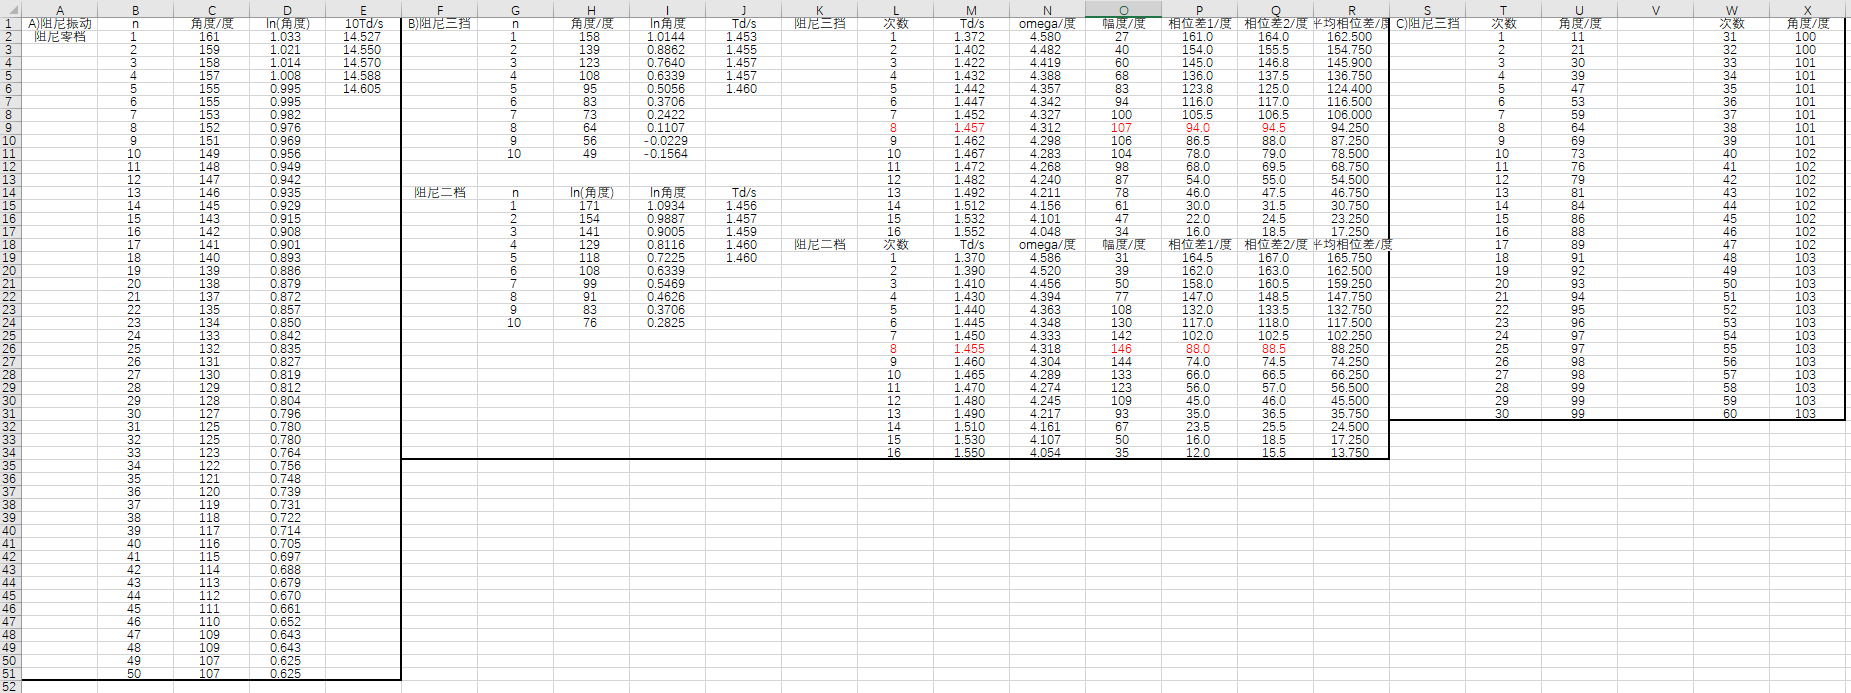
\includegraphics[scale=0.5]{data1.PNG}
\end{center}\vspace{0mm}
\begin{flushright}
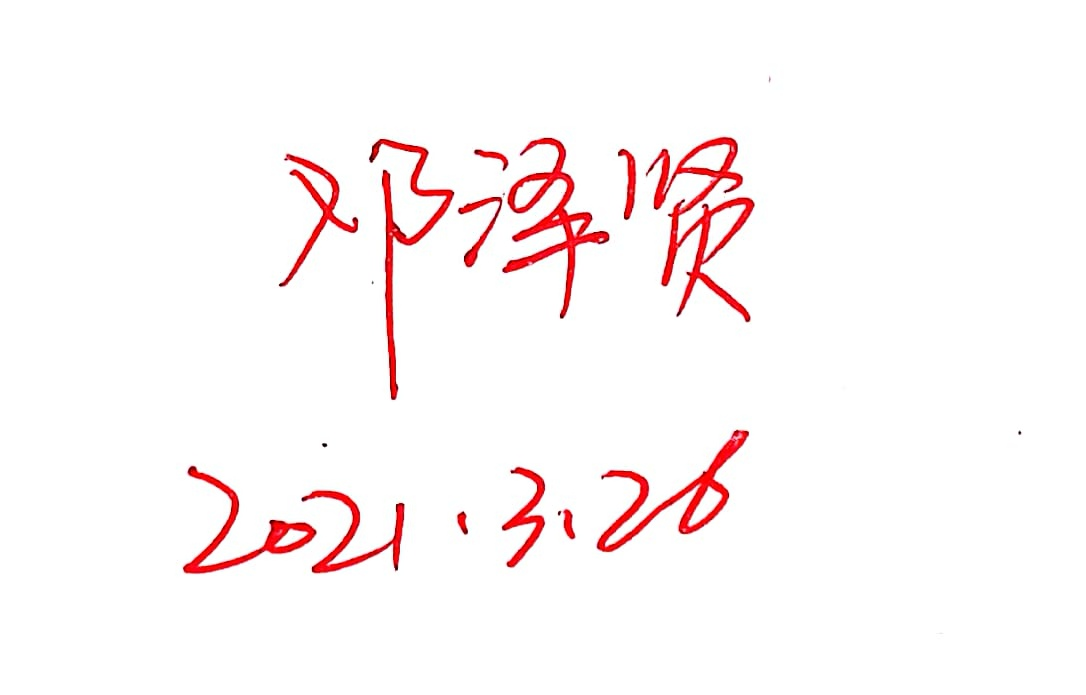
\includegraphics[scale=0.10]{data2.jpg}\end{flushright}
\end{figure}
\end{document}